\documentclass[12pt,a4paper]{article}

\usepackage[utf8]{inputenc}
\usepackage[portuguese]{babel}
\usepackage[margin=2.5cm]{geometry}
\usepackage{graphicx}
\usepackage{booktabs}
\usepackage{tabularx}
\usepackage{hyperref}
\usepackage{amsmath}
\usepackage{float}
\usepackage{caption}
\usepackage{subcaption}
\usepackage{xcolor}
\usepackage[numbers]{natbib}

\hypersetup{
  colorlinks=true,
  linkcolor=blue,
  citecolor=blue,
  urlcolor=blue
}

\title{Avaliação de Performance e Consumo Energético de C\# em Windows e Linux:\\
Um Estudo Comparativo com FannkuchRedux e BinaryTrees}
\author{Gustavo Castro\\
\small Universidade do Minho, Departamento de Informática\\
\small Mestrado em Engenharia Informática}
\date{Maio de 2026}

\begin{document}

\maketitle
\tableofcontents
\newpage

%% ─────────────────────────────────────────────────────────────────────────────
\section{Resumo}
%% ─────────────────────────────────────────────────────────────────────────────

Este trabalho compara a performance e o consumo energético de C\# em Windows 11 e
Ubuntu 24.04 utilizando dois \textit{benchmarks} complementares: FannkuchRedux,
CPU-bound, e BinaryTrees, GC-bound / memory-bound.
A medição de energia foi realizada diretamente via Intel RAPL
(\textit{Running Average Power Limit}) nos domínios \textit{Package} e DRAM,
a medição de tempo via BenchmarkDotNet, e ambos os sistemas operativos correram
no mesmo hardware (\textit{dual-boot}), com turbo desativado para garantir
comparabilidade.

Em FannkuchRedux, Windows é 43.4\% mais rápido para N=11 e 37.7\% mais rápido
para N=12, mas Linux consome 35\% menos energia para N=11 (17.4\,J vs.\
27.0\,J) e 17\% menos para N=12 (232.2\,J vs.\ 281.4\,J).
Em BinaryTrees, Windows é 23\% mais rápido para N=16 (148\,ms vs.\ 192\,ms) e
11\% mais rápido para N=18 (1108\,ms vs.\ 1246\,ms), enquanto Linux consome
51\% menos energia para N=16 (2.1\,J vs.\ 4.3\,J) e 56\% menos para N=18
(12.9\,J vs.\ 29.1\,J).

A medição independente do domínio DRAM confirma o perfil de cada
\textit{workload}: em FannkuchRedux a DRAM representa apenas 2.7\% (Linux) /
1.3\% (Windows) da energia do \textit{Package}, ao passo que em BinaryTrees
sobe para 10.6\% (Linux) / 5.0\% (Windows), uma razão 4--8$\times$ superior
que confirma experimentalmente a natureza GC-bound do segundo
\textit{benchmark}.
Todas as diferenças relevantes são estatisticamente significativas
(Mann-Whitney U, $p < 0.001$), confirmadas por testes de permutação
independentes.
Conclui-se que existe um \textit{trade-off} claro entre velocidade e
eficiência energética entre os dois sistemas operativos, com magnitude
dependente do perfil de memória do \textit{workload}, com implicações
práticas para decisões de \textit{deployment} em ambientes onde o custo
energético é relevante.

%% ─────────────────────────────────────────────────────────────────────────────
\section{Introdução}
%% ─────────────────────────────────────────────────────────────────────────────

A eficiência energética do software é uma preocupação crescente, especialmente em
contextos de computação de alto desempenho e \textit{edge computing}.
A linguagem C\# e o ecossistema .NET são amplamente usados em ambientes de
produção que correm tanto em Windows como em Linux.
Compreender como o sistema operativo influencia a performance e o consumo
energético de um mesmo programa é relevante para decisões de \textit{deployment}.

A maioria dos estudos de performance em .NET foca-se em métricas de tempo de
execução, ignorando o consumo energético.
Estudos como o de Pereira et al.\ \cite{Pereira2017}
(\textit{greensoftwarelab/Energy-Languages} \cite{EnergyLanguages}) demonstram
que a linguagem e o ambiente de execução têm impacto significativo na energia
consumida.
Este trabalho estende essa linha de investigação para comparar dois sistemas
operativos com o mesmo hardware e \textit{runtime}.

Para evitar que as conclusões dependam de um único perfil de \textit{workload},
o estudo combina dois \textit{benchmarks} complementares.
FannkuchRedux fornece o caso CPU-bound puro (alocação de \textit{heap}
desprezável, contenda dominada por aritmética e acesso a \textit{arrays}).
BinaryTrees foi adicionado como contraponto GC-bound: a alocação de
\textit{heap} é de aproximadamente 227\,MB (N=16) a 1037\,MB (N=18) por
iteração, exercitando intensamente o coletor de lixo e o subsistema de
memória.
Esta combinação permite distinguir efeitos do \textit{scheduler} e do JIT
(visíveis sobretudo em FannkuchRedux) de efeitos do GC e da pressão sobre o
subsistema DRAM (visíveis sobretudo em BinaryTrees).
Para validar experimentalmente este perfil de memória, o subsistema DRAM é
medido de forma independente via Intel RAPL, em adição ao domínio
\textit{Package}.

Este trabalho tem como objetivos:
(1) medir e comparar o tempo de execução de C\# em Windows 11 e Ubuntu 24.04;
(2) medir e comparar o consumo energético via Intel RAPL em ambos os sistemas
operativos;
(3) avaliar a significância estatística das diferenças observadas;
(4) comparar \textit{workloads} CPU-bound (FannkuchRedux) com \textit{workloads}
GC-bound (BinaryTrees);
(5) medir o subsistema DRAM via Intel RAPL para caracterizar experimentalmente
o perfil de memória de cada \textit{benchmark}.

O restante documento está organizado da seguinte forma: a Secção~\ref{sec:metodologia}
descreve a metodologia e o ambiente experimental; a Secção~\ref{sec:resultados}
apresenta os resultados obtidos; a Secção~\ref{sec:discussao} discute as
implicações dos resultados; a Secção~\ref{sec:ameacas} identifica ameaças à
validade; a Secção~\ref{sec:conclusao} conclui o trabalho.

%% ─────────────────────────────────────────────────────────────────────────────
\section{Metodologia}
\label{sec:metodologia}
%% ─────────────────────────────────────────────────────────────────────────────

\subsection{Algoritmos de Benchmark}
\label{sec:algoritmos}

\subsubsection{FannkuchRedux (CPU-bound)}

O FannkuchRedux é um algoritmo CPU-bound puro, sem I/O, baseado em permutações
de arrays, proveniente do \textit{Computer Language Benchmarks Game} (CLBG)
\cite{CLBG}.
A implementação em C\# utilizada é a referência de
\textit{greensoftwarelab/Energy-Languages} \cite{EnergyLanguages}, contribuída
por Isaac Gouy, transliterada do programa Java de Oleg Mazurov, com melhorias de
concorrência por Peperud \cite{Pereira2017}.

Foram testadas duas variantes: N=11 e N=12 (tamanho do problema, que determina
a complexidade fatorial).
O algoritmo utiliza \textit{threading} via \texttt{Task.Run} com
\texttt{Environment.ProcessorCount + 1} \textit{workers}.
A correção foi verificada: \texttt{Compute(7)} devolve \textit{checksum} 228 e
\textit{maxFlips} 16, correspondendo ao valor de referência do CLBG.
A alocação de \textit{heap} é de aproximadamente 52\,KB por iteração (verificado
via \texttt{MemoryDiagnoser} do BenchmarkDotNet), pelo que o GC é irrelevante
para os resultados.

\subsubsection{BinaryTrees (GC-bound / Memory-bound)}

O BinaryTrees é um algoritmo GC-bound proveniente do CLBG \cite{CLBG} que
aloca e percorre árvores binárias recursivas, exercitando intensamente o
coletor de lixo e o subsistema de memória.
A implementação em C\# utilizada é a referência de
\textit{greensoftwarelab/Energy-Languages} \cite{EnergyLanguages}, contribuída
por Marek Safar, com melhorias de concorrência por Peperud.

Foram testadas duas variantes: N=16 e N=18.
A alocação de \textit{heap} é de aproximadamente 227\,MB para N=16 e 1037\,MB
para N=18 por iteração, ordens de magnitude superior à de FannkuchRedux,
o que torna o subsistema de memória o componente dominante do consumo
energético.
O algoritmo utiliza \textit{threading} via \texttt{Task.Run} com
\textit{work-stealing} e paralelismo adaptativo (sobre-paralelização para
profundidades elevadas).
A correção foi verificada: \texttt{Compute(10)} devolve
\textit{stretchCheck}~$=4095$ e \textit{longLivedCheck}~$=2047$,
correspondendo ao valor de referência do CLBG.

\subsection{Hardware e Software}

A Tabela~\ref{tab:hardware} resume as especificações do ambiente de teste.

\begin{table}[H]
  \centering
  \caption{Especificações de hardware e software do ambiente de teste.}
  \label{tab:hardware}
  \begin{tabular}{ll}
    \toprule
    \textbf{Campo} & \textbf{Valor} \\
    \midrule
    Máquina        & HP EliteBook 1050 G1 \\
    CPU            & Intel Core i7-8850H (Coffee Lake, 6C/12T, 2.6\,GHz base) \\
    RAM            & 16\,GiB \\
    Armazenamento  & Samsung NVMe 512\,GB \\
    SO Linux       & Ubuntu 24.04.3 LTS, kernel 6.17.0-22-generic \\
    SO Windows     & Windows 11 Pro (build 26200.8246) \\
    .NET SDK       & 9.0.312 (Linux) / 9.0.313 (Windows) \\
    Runtime .NET   & 9.0.14 (Linux) / 9.0.15 (Windows) \\
    BenchmarkDotNet & 0.15.8 \\
    \bottomrule
  \end{tabular}
\end{table}

\subsection{Medição de Performance --- BenchmarkDotNet}

A ferramenta BenchmarkDotNet 0.15.8 \cite{BenchmarkDotNet} foi usada para medir
o tempo de execução.
A configuração incluiu \texttt{SimpleJob(RuntimeMoniker.Net90)},
\texttt{MemoryDiagnoser} e \texttt{CsvMeasurementsExporter}.
O aquecimento (\textit{warm-up}) é realizado automaticamente antes das iterações
medidas, com deteção e remoção automática de \textit{outliers} estatísticos pelo
BenchmarkDotNet.
A compilação foi feita em modo \textit{Release}, x64, com
\texttt{Optimize=true}.
Em Windows foi usado \texttt{InProcessEmitToolchain} (necessário para a
integração com a LibreHardwareMonitorLib).

\subsection{Medição de Energia --- Intel RAPL}
\label{sec:rapl}

A energia foi medida via Intel RAPL \cite{IntelRAPL} em três domínios:
\textit{Package} (\texttt{MSR\_PKG\_ENERGY\_STATUS}, 0x611), que inclui todos
os núcleos e o \textit{uncore}; PP0/\textit{Cores}
(\texttt{MSR\_PP0\_ENERGY\_STATUS}, 0x639); e DRAM
(\texttt{MSR\_DRAM\_ENERGY\_STATUS}, 0x619), que isola o consumo do
subsistema de memória.
A inclusão do domínio DRAM permite caracterizar experimentalmente o perfil de
memória de cada \textit{benchmark} (ver Secção~\ref{sec:dram}).

\textbf{Linux:} leitura via sysfs (\textit{kernel powercap}), com os caminhos:
\begin{itemize}
  \item Package:
    \texttt{/sys/devices/virtual/powercap/intel-rapl/intel-rapl:0/energy\_uj}
  \item PP0/Cores:
    \texttt{/sys/devices/virtual/powercap/intel-rapl/intel-rapl:0/intel-rapl:0:0/energy\_uj}
  \item DRAM:
    \texttt{/sys/devices/virtual/powercap/intel-rapl/intel-rapl:0/intel-rapl:0:2/energy\_uj}
\end{itemize}

\textbf{Windows:} leitura via driver WinRing0 (LibreHardwareMonitorLib 0.9.3)
\cite{LibreHardwareMonitor}, com acesso direto ao MSR por reflexão sobre
\texttt{LibreHardwareMonitor.Hardware.Ring0.ReadMsr} para os três domínios
(\texttt{0x611}, \texttt{0x639}, \texttt{0x619}).

A unidade de energia é lida do \texttt{MSR\_RAPL\_POWER\_UNIT} (0x606),
bits [12:8] --- para Coffee Lake: $2^{-14}$\,J/unit $\approx$ 61\,µJ/unit, com
o mesmo multiplicador a aplicar-se a todos os três domínios.
O método de medição consiste na leitura dos contadores antes e depois de cada
iteração; o delta é a energia consumida.
O \textit{wraparound} dos contadores de 32 bits foi tratado (período de
\textit{wrap} muito superior à duração das \textit{runs}).
O CSV de saída inclui as colunas \texttt{pkg\_energy\_uj}, \texttt{pp0\_energy\_uj}
e \texttt{dram\_energy\_uj}, além de \textit{timestamp}, duração (ms) e
temperatura.

\subsection{Configuração do Ambiente de Medição}

Para garantir comparabilidade entre os dois sistemas operativos, as seguintes
configurações foram aplicadas:

\textbf{Ambos os SO:}
\begin{itemize}
  \item Turbo Boost desativado
    (Linux: \texttt{/sys/devices/system/cpu/intel\_pstate/no\_turbo=1};
    Windows: \texttt{PROCTHROTTLEMAX=99\%})
  \item Máquina ligada à corrente (AC power)
  \item Sem outras aplicações intensivas em CPU durante as medições
\end{itemize}

\textbf{Linux:}
\begin{itemize}
  \item CPU governor: \texttt{performance} (via cpupower)
  \item Script de lançamento: \texttt{scripts/run-linux.sh}
\end{itemize}

\textbf{Windows:}
\begin{itemize}
  \item Plano de energia: Desempenho Máximo (GUID \texttt{202e5b95\ldots})
  \item Processo executado como Administrador (necessário para acesso MSR via
    WinRing0)
\end{itemize}

\subsection{Protocolo de Recolha de Dados}

O número de iterações foi determinado automaticamente pelo BenchmarkDotNet
(mínimo de estabilidade estatística).
As amostras válidas, após remoção de \textit{outliers} (critério IQR 1.5×),
foram:
\begin{itemize}
  \item FannkuchRedux: Linux N=11: 25 amostras; Linux N=12: 24 amostras;
    Windows N=11: 23 amostras; Windows N=12: 19 amostras
  \item BinaryTrees: Linux N=16: 80 amostras; Linux N=18: 22 amostras;
    Windows N=16: 123 amostras; Windows N=18: 49 amostras
\end{itemize}
Os dados foram exportados para CSV com \textit{timestamp}, energia (µJ) nos
domínios Package/PP0/DRAM, duração (ms) e temperatura.

\subsection{Análise Estatística}

Foram utilizados os seguintes testes e medidas:
\begin{itemize}
  \item \textbf{Mann-Whitney U} (amostras independentes, não-paramétrico)
  \item \textbf{A/B test por permutação} (10\,000 permutações)
  \item \textbf{Correlação de Spearman} $\rho$ (relação não-linear entre tempo
    e energia)
  \item \textbf{Intervalos de confiança} a 95\%, calculados via distribuição
    $t$ de Student
\end{itemize}
O nível de significância foi $\alpha = 0.05$.
As ferramentas utilizadas foram Python 3, pandas, scipy, seaborn e matplotlib.

%% ─────────────────────────────────────────────────────────────────────────────
\section{Resultados}
\label{sec:resultados}
%% ─────────────────────────────────────────────────────────────────────────────

A Tabela~\ref{tab:estatisticas} apresenta as estatísticas descritivas
completas para os oito grupos experimentais (dois algoritmos $\times$ dois
valores de N $\times$ dois SO).

\begin{table}[H]
  \centering
  \caption{Estatísticas descritivas por algoritmo, SO e valor de N.}
  \label{tab:estatisticas}
  \footnotesize
  \begin{tabular}{lllrrrrrrr}
    \toprule
    \textbf{Algoritmo} & \textbf{SO} & \textbf{N} & \textbf{n} &
    \textbf{Média (ms)} & \textbf{DP (ms)} & \textbf{CV (\%)} &
    \textbf{Pkg (J)} & \textbf{DRAM (J)} & \textbf{DRAM/Pkg (\%)} \\
    \midrule
    FannkuchRedux & Linux   & 11 & 25  & 643.0   & 11.20 & 1.74 & 17.424  & 0.484 & 2.78  \\
    FannkuchRedux & Linux   & 12 & 24  & 8663.9  & 27.68 & 0.32 & 232.162 & 6.221 & 2.68  \\
    FannkuchRedux & Windows & 11 & 23  & 448.3   & 3.79  & 0.84 & 27.013  & 0.319 & 1.18  \\
    FannkuchRedux & Windows & 12 & 19  & 6293.9  & 38.92 & 0.62 & 281.436 & 3.724 & 1.32  \\
    BinaryTrees   & Linux   & 16 & 80  & 192.4   & 8.60  & 4.47 & 2.097   & 0.212 & 10.13 \\
    BinaryTrees   & Linux   & 18 & 22  & 1246.1  & 20.89 & 1.68 & 12.878  & 1.425 & 11.07 \\
    BinaryTrees   & Windows & 16 & 123 & 148.3   & 8.87  & 5.98 & 4.305   & 0.214 & 4.97  \\
    BinaryTrees   & Windows & 18 & 49  & 1107.8  & 30.54 & 2.76 & 29.088  & 1.463 & 5.03  \\
    \bottomrule
  \end{tabular}
\end{table}

\subsection{FannkuchRedux (CPU-bound)}
\label{sec:res_fannkuch}

\subsubsection{Visualização dos Dados}

A Figura~\ref{fig:boxplot_time} mostra a distribuição do tempo de execução por
SO e N para FannkuchRedux.

\begin{figure}[H]
  \centering
  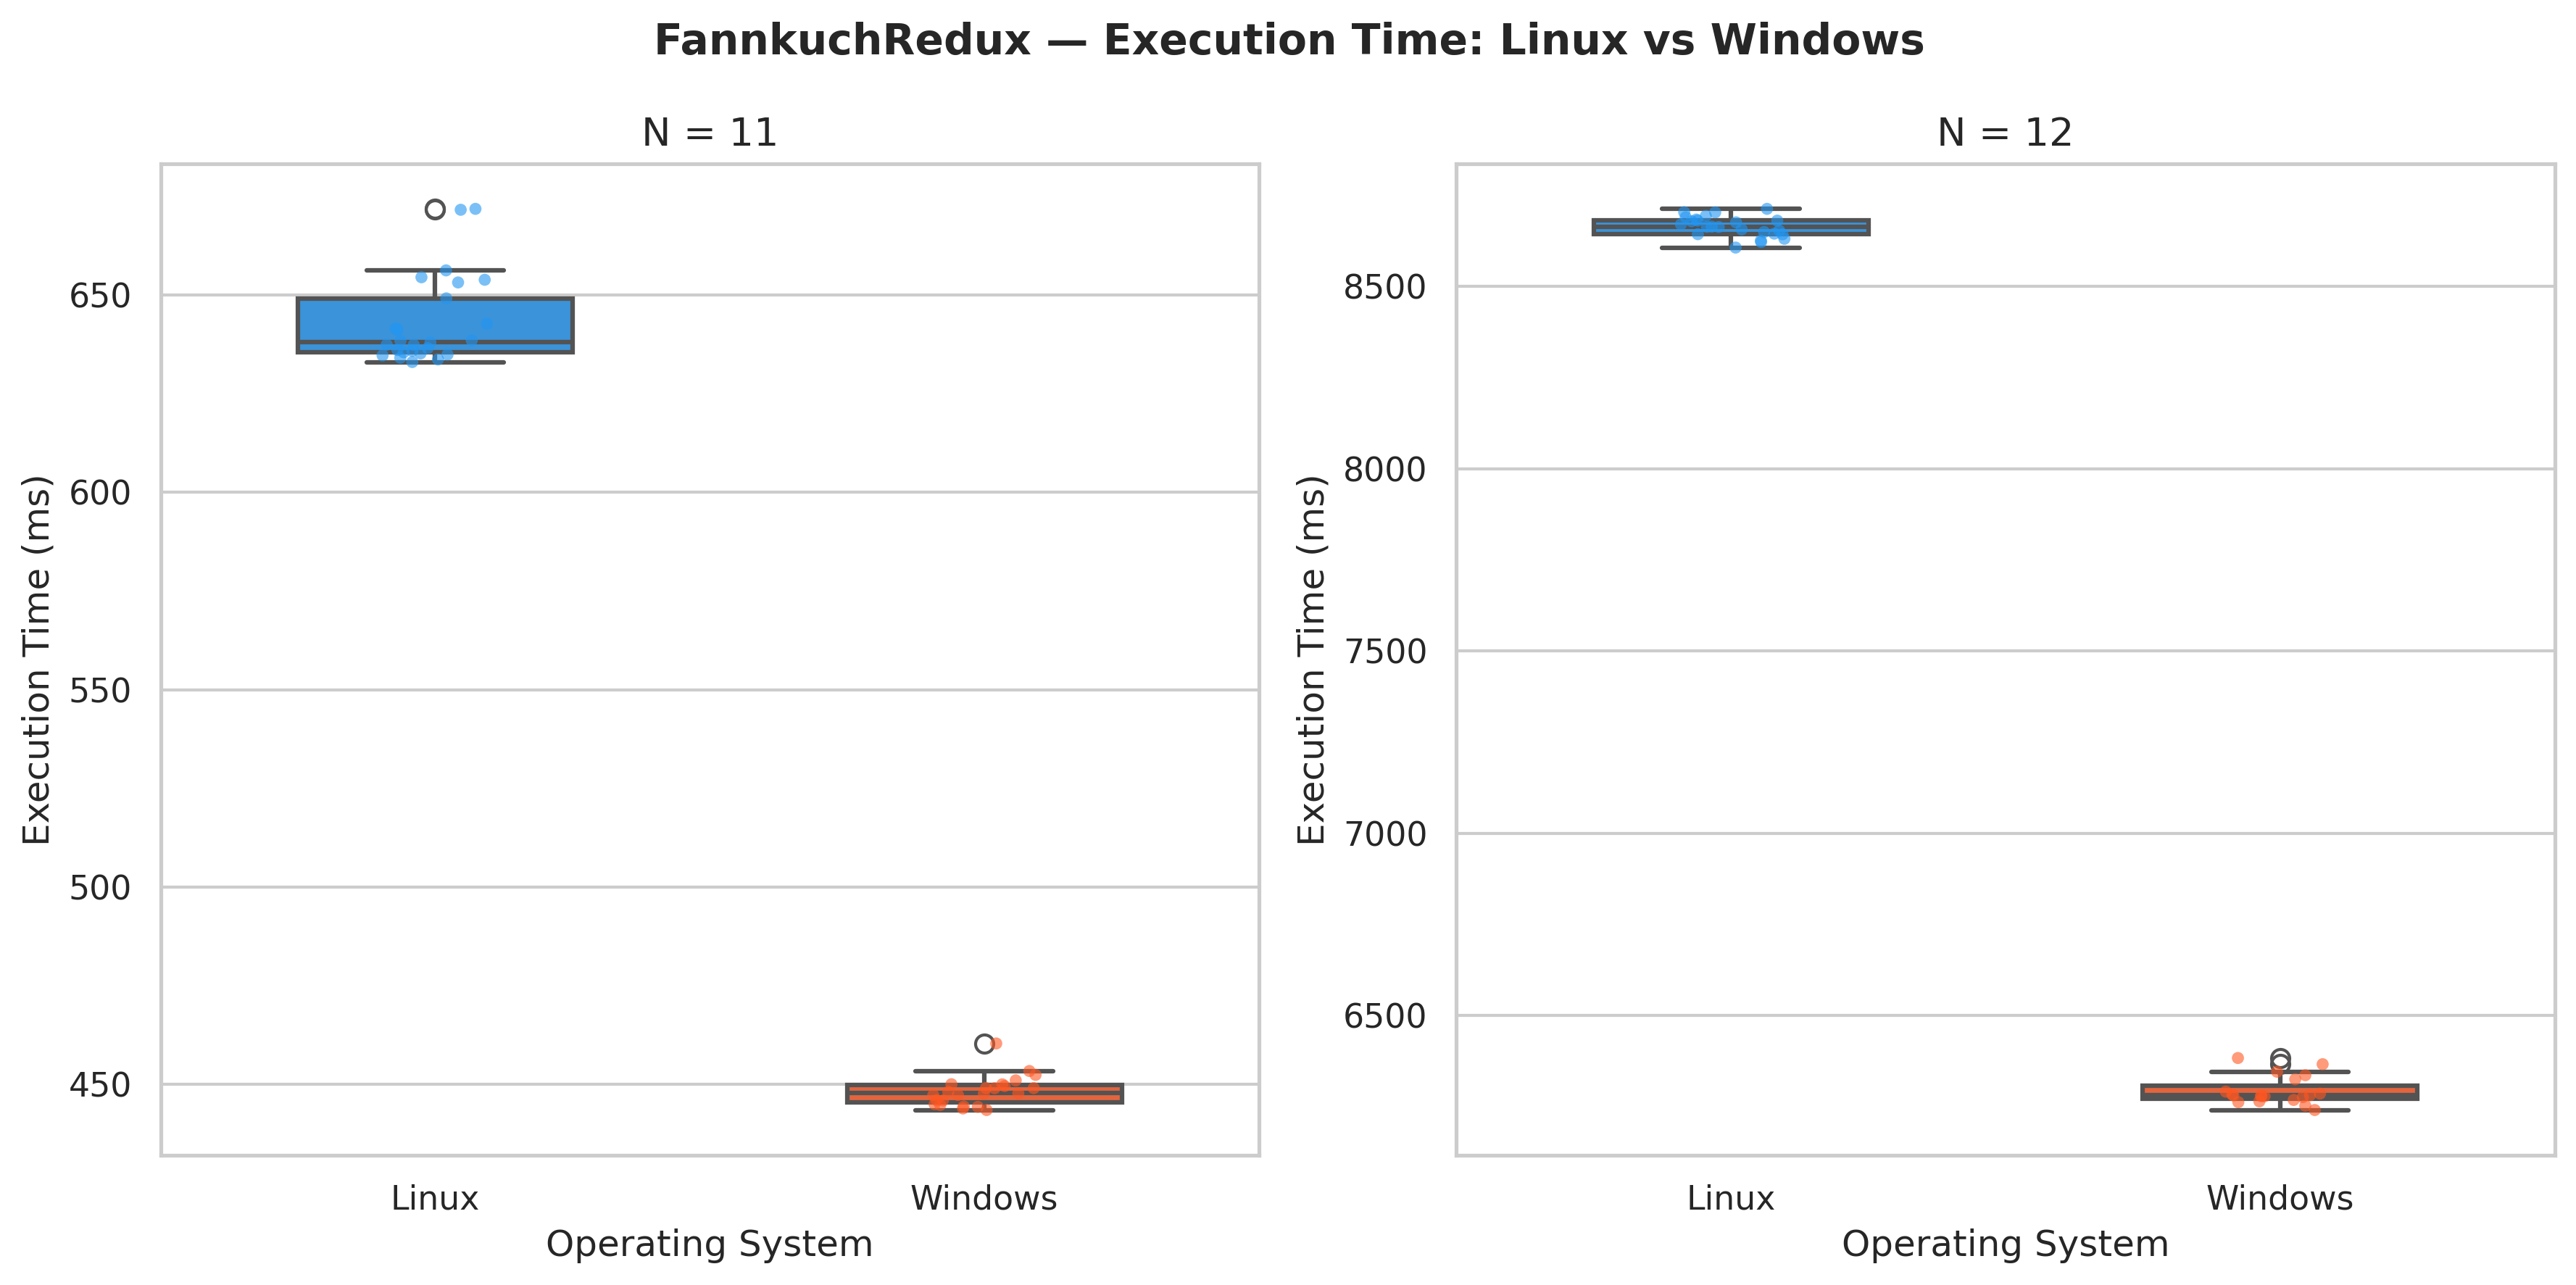
\includegraphics[width=\textwidth]{../analysis/figures/01_boxplot_time.png}
  \caption{FannkuchRedux: distribuição do tempo de execução para N=11 e N=12 em
    Linux e Windows. Os pontos representam iterações individuais.}
  \label{fig:boxplot_time}
\end{figure}

A Figura~\ref{fig:boxplot_energy} apresenta a distribuição do consumo
energético (domínio \textit{Package}) por SO e N.

\begin{figure}[H]
  \centering
  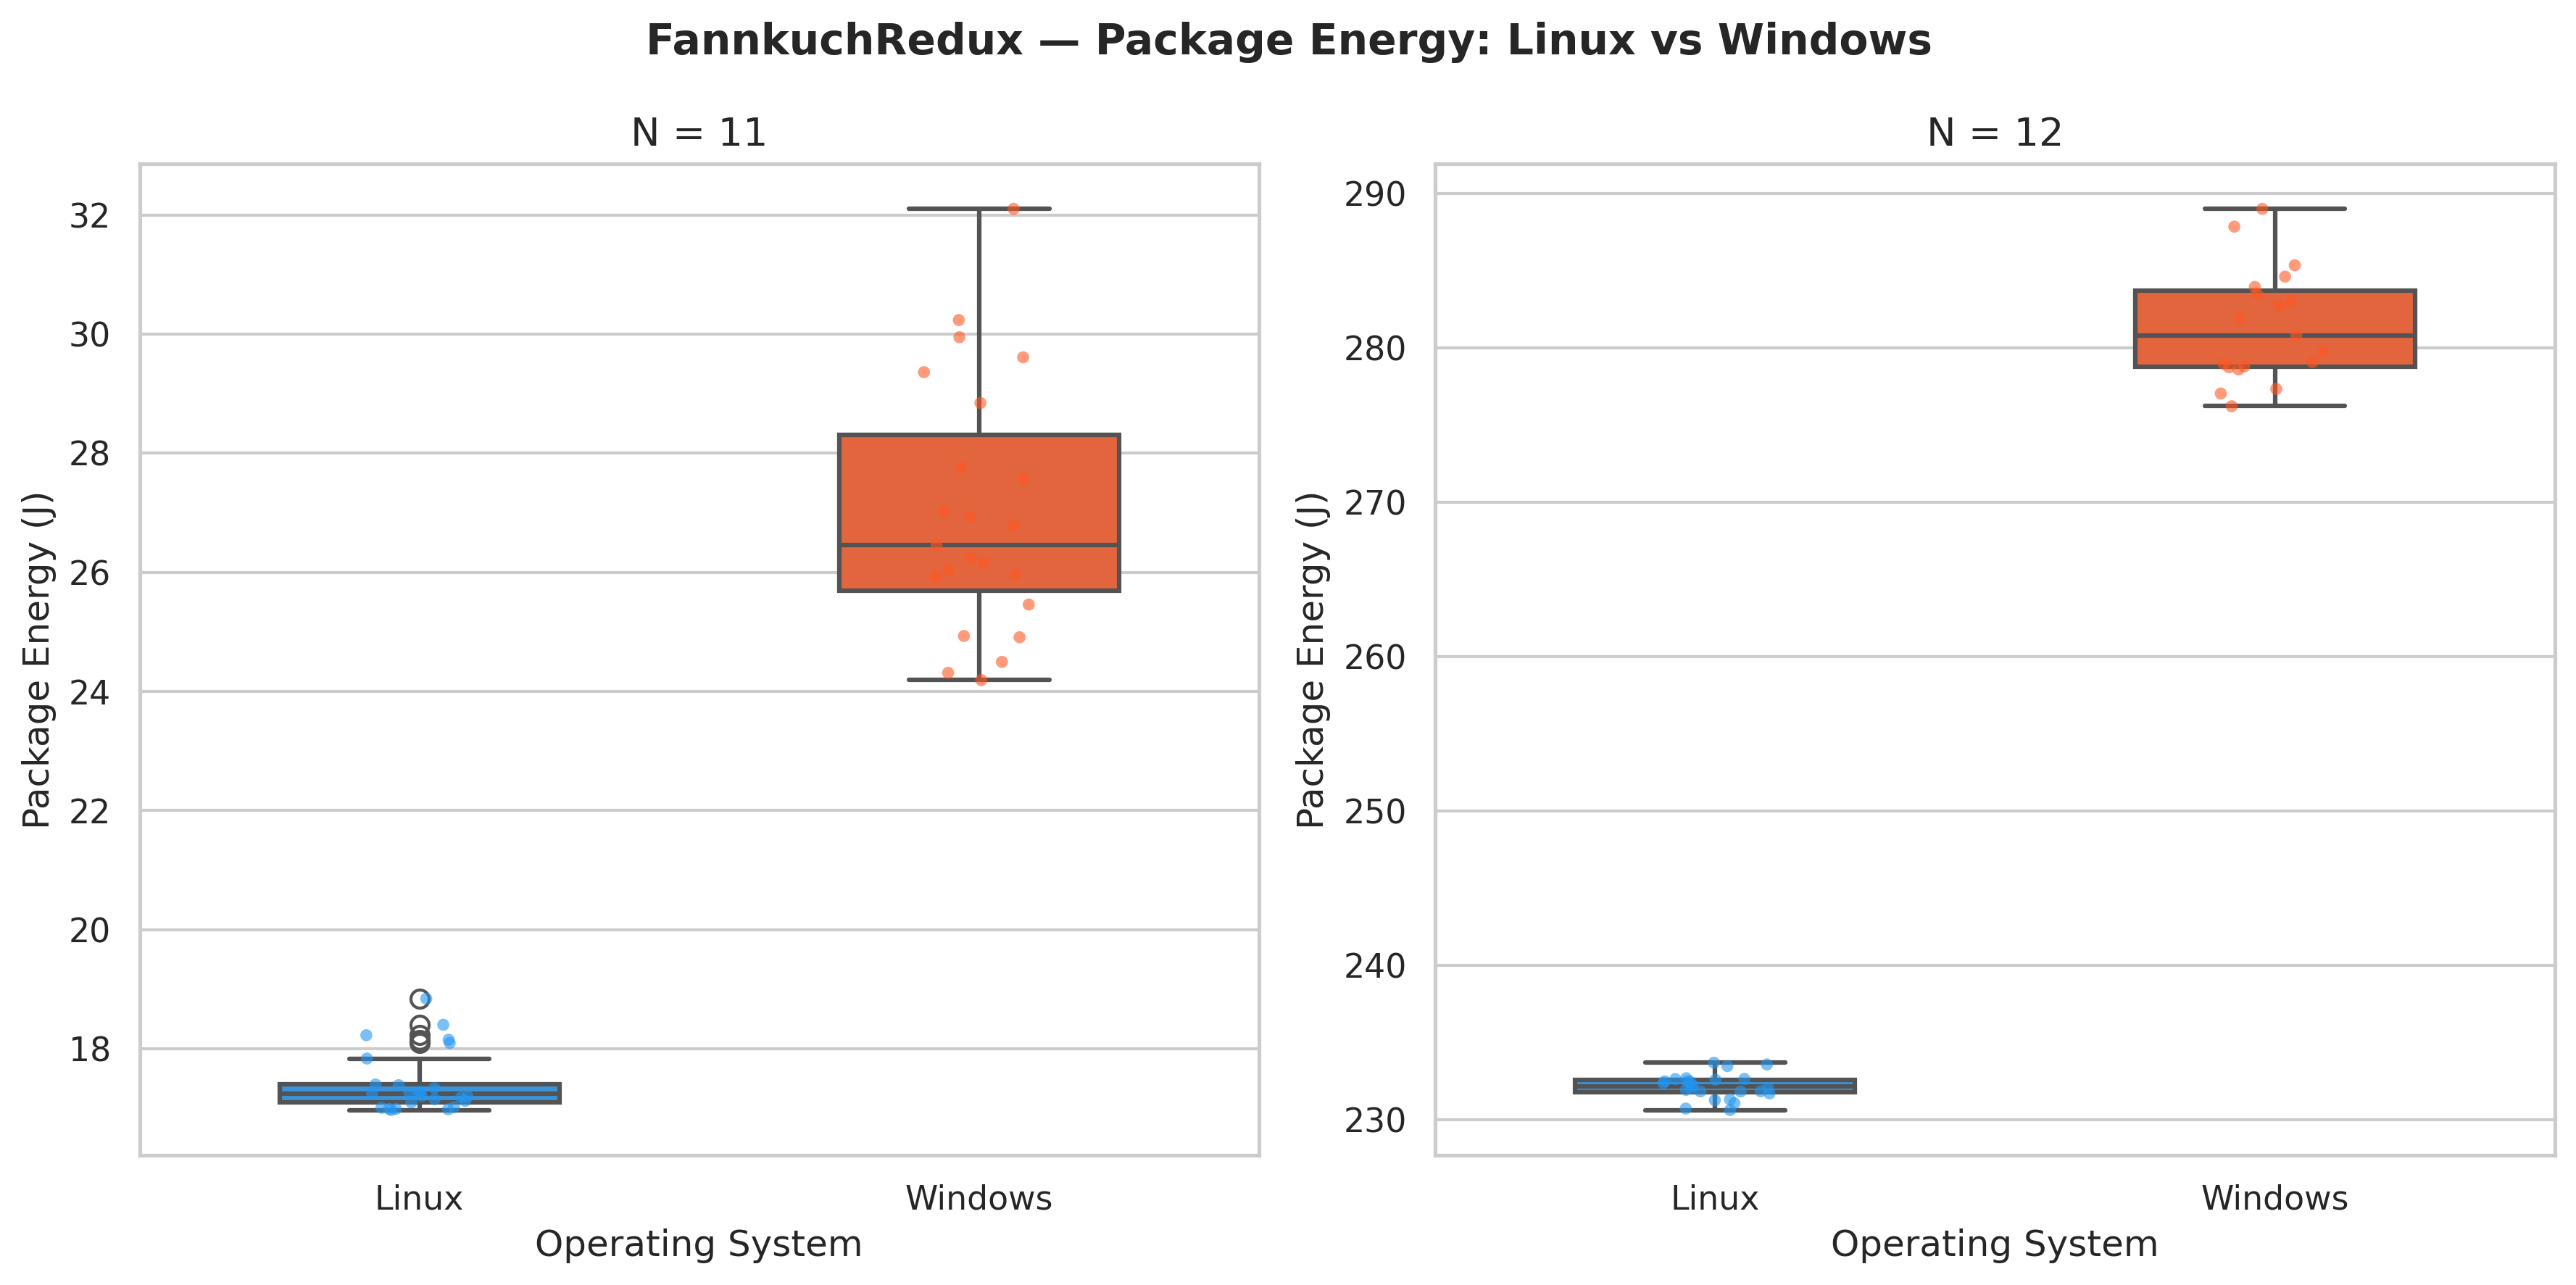
\includegraphics[width=\textwidth]{../analysis/figures/02_boxplot_energy.png}
  \caption{FannkuchRedux: distribuição do consumo energético (domínio
    \textit{Package}) para N=11 e N=12.}
  \label{fig:boxplot_energy}
\end{figure}

A Figura~\ref{fig:summary_bar} apresenta as médias e intervalos de confiança a
95\% para tempo de execução e energia.

\begin{figure}[H]
  \centering
  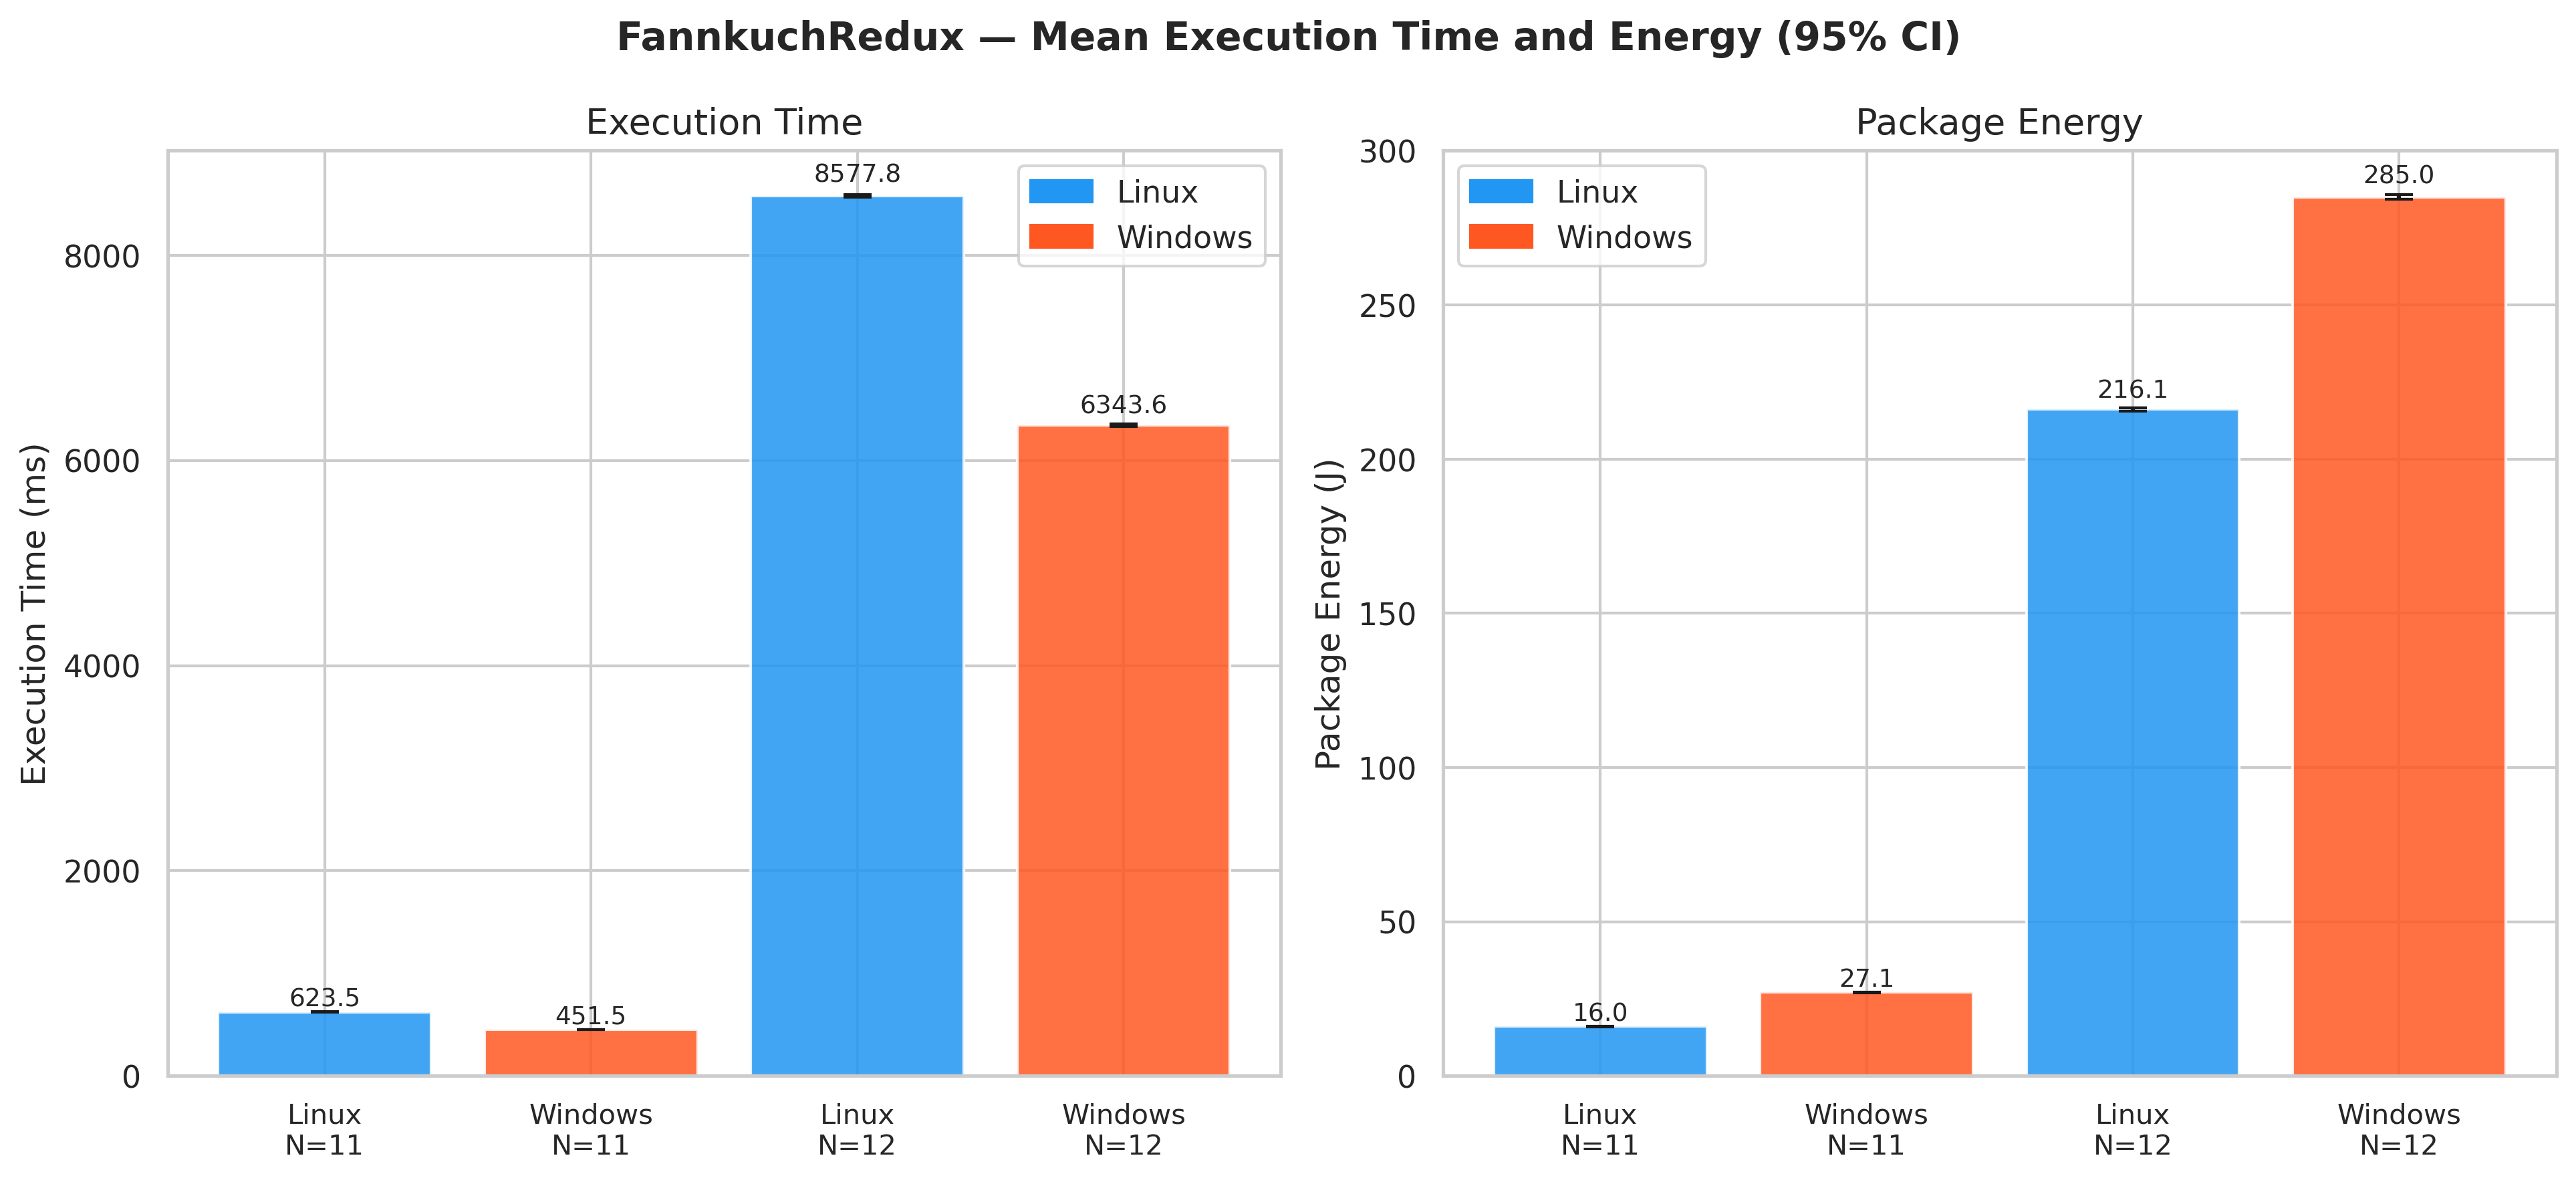
\includegraphics[width=\textwidth]{../analysis/figures/06_summary_bar.png}
  \caption{FannkuchRedux: média e IC 95\% para tempo de execução (esq.) e
    energia (dir.) por SO e N.}
  \label{fig:summary_bar}
\end{figure}

A Figura~\ref{fig:histogram_time} mostra a distribuição do tempo de execução
por SO e N (histograma com KDE sobreposto).

\begin{figure}[H]
  \centering
  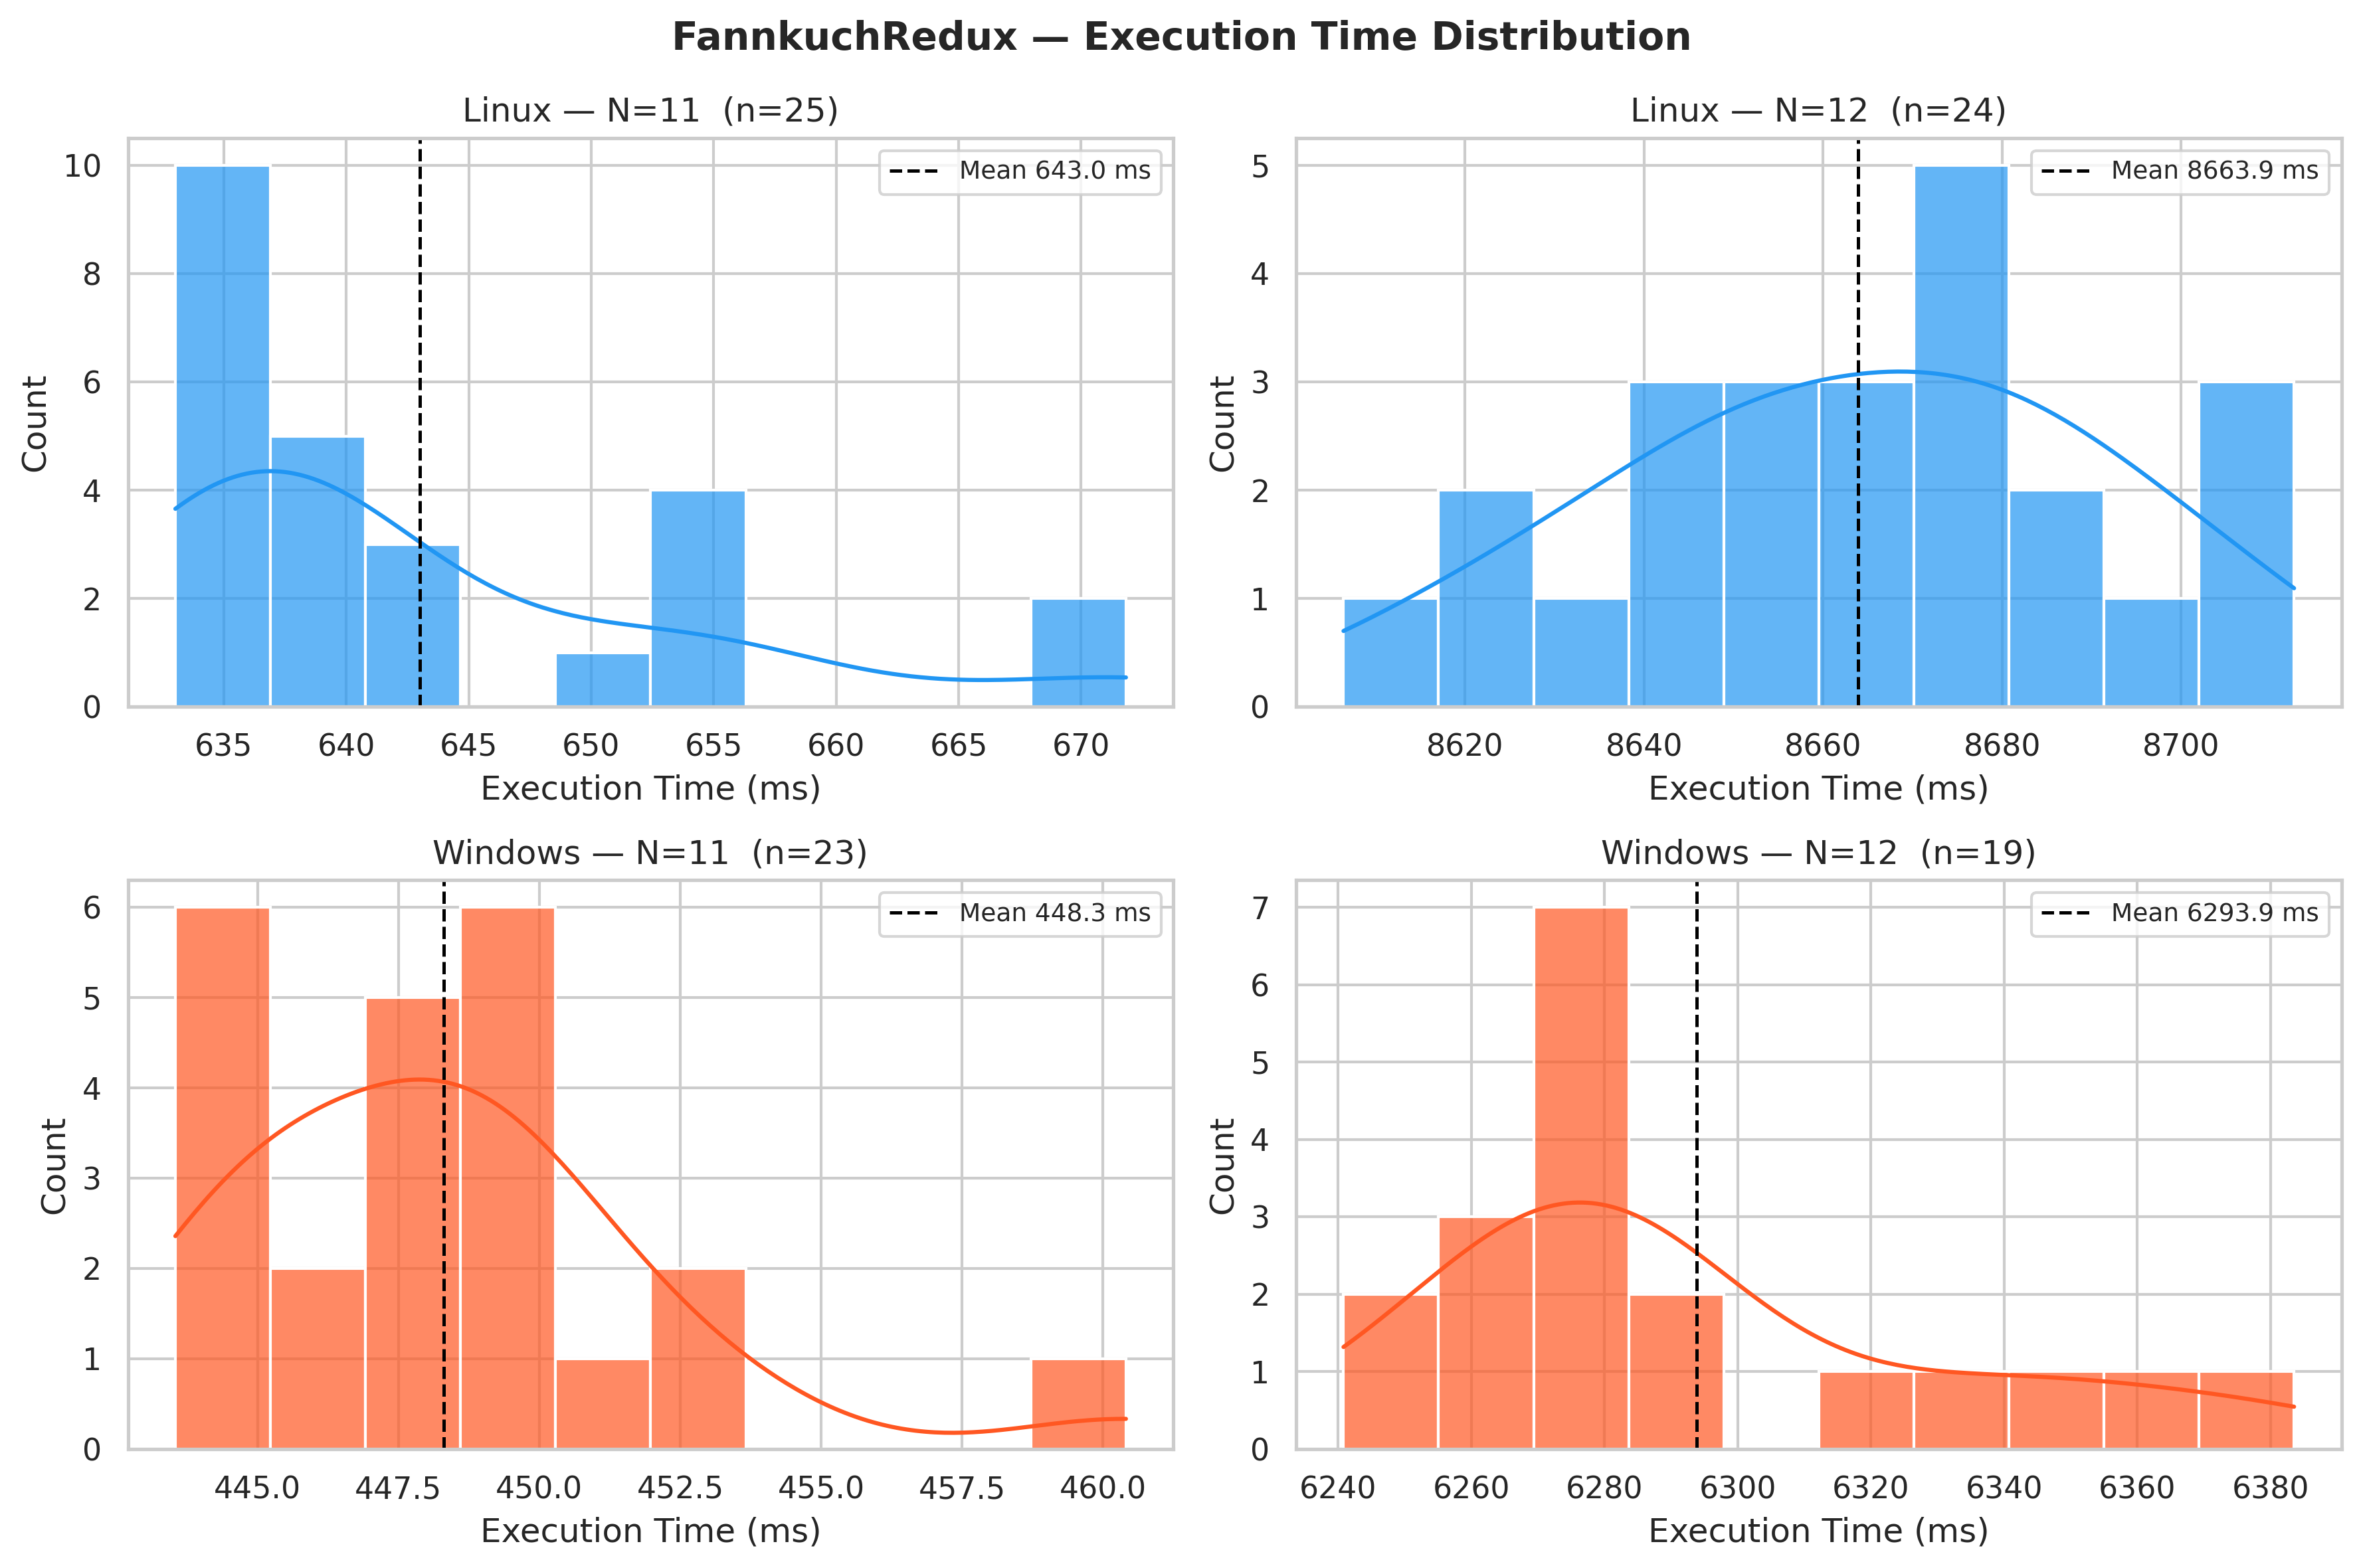
\includegraphics[width=\textwidth]{../analysis/figures/03_histogram_time.png}
  \caption{FannkuchRedux: distribuição do tempo de execução por SO e N
    (histograma + KDE).}
  \label{fig:histogram_time}
\end{figure}

\subsubsection{Comparação de Performance (Tempo)}

Para N=11, Windows executa em 448.3\,ms (IC 95\%: [446.7, 449.9]\,ms) vs.\
Linux 643.0\,ms (IC 95\%: [638.4, 647.6]\,ms).
\textbf{Windows é 43.4\% mais rápido.}
Os intervalos de confiança não se sobrepõem.

Para N=12, Windows executa em 6293.9\,ms (IC 95\%: [6275.1, 6312.6]\,ms) vs.\
Linux 8663.9\,ms (IC 95\%: [8652.2, 8675.6]\,ms).
\textbf{Windows é 37.7\% mais rápido.}

\subsubsection{Comparação de Consumo Energético}

Para N=11, Linux consome 17.424\,J (IC 95\%: [17.211, 17.638]\,J) vs.\ Windows
27.013\,J (IC 95\%: [26.095, 27.931]\,J).
\textbf{Linux consome 35.5\% menos energia.}

Para N=12, Linux consome 232.162\,J (IC 95\%: [231.820, 232.504]\,J) vs.\
Windows 281.436\,J (IC 95\%: [279.680, 283.193]\,J).
\textbf{Linux consome 17.5\% menos energia.}

\subsubsection{Significância Estatística}

A Tabela~\ref{tab:testes_fr} apresenta os resultados dos testes de hipótese
para FannkuchRedux.
Todas as diferenças são estatisticamente significativas com $p < 0.001$
($\alpha = 0.05$).

\begin{table}[H]
  \centering
  \caption{FannkuchRedux: resultados dos testes de hipótese para tempo e
    energia.}
  \label{tab:testes_fr}
  \begin{tabular}{llllll}
    \toprule
    \textbf{N} & \textbf{Métrica} & \textbf{Teste} & \textbf{Estatística} &
    \textbf{p-value} & \textbf{Significativo} \\
    \midrule
    11 & Tempo   & Mann-Whitney U  & 575.0          & 3.16e-9  & Sim (***) \\
    11 & Energia & Mann-Whitney U  & 0.0            & 1.58e-9  & Sim (***) \\
    11 & Tempo   & Permutação A/B  & 194.7\,ms      & $<$0.001 & Sim (***) \\
    11 & Energia & Permutação A/B  & $-$9.59\,J     & $<$0.001 & Sim (***) \\
    12 & Tempo   & Mann-Whitney U  & 456.0          & 2.64e-8  & Sim (***) \\
    12 & Energia & Mann-Whitney U  & 0.0            & 1.32e-8  & Sim (***) \\
    12 & Tempo   & Permutação A/B  & 2370.0\,ms     & $<$0.001 & Sim (***) \\
    12 & Energia & Permutação A/B  & $-$49.27\,J    & $<$0.001 & Sim (***) \\
    \bottomrule
  \end{tabular}
\end{table}

\subsubsection{Correlação Tempo--Energia}

A correlação de Spearman entre tempo de execução e energia consumida é forte e
estatisticamente significativa em ambos os grupos:
\begin{itemize}
  \item Spearman $\rho$ (FannkuchRedux completo) $= 0.596$, $p < 0.001$
  \item Spearman $\rho$ (Linux) $= 0.933$, $p < 0.001$
  \item Spearman $\rho$ (Windows) $= 0.818$, $p < 0.001$
\end{itemize}

A correlação por SO é muito forte ($\rho > 0.8$ em ambos), o esperado para um
\textit{workload} CPU-bound puro.
A correlação combinada é mais baixa porque agrega dois SO com regimes
energia/tempo distintos.

\subsubsection{Variância e Estabilidade}

O coeficiente de variação (CV) do Linux mantém-se baixo (0.32\%--1.74\%),
indicando ambiente de medição muito estável.
O CV do Windows N=11 (0.84\%) é ligeiramente inferior ao CV do Linux N=11
(1.74\%) neste \textit{dataset}, ao passo que para N=12 ambos os SO descem
para CV inferior a 1\%, sugerindo que \textit{workloads} mais longas
estabilizam o comportamento de medição.

\subsection{BinaryTrees (GC-bound / Memory-bound)}
\label{sec:res_bt}

\subsubsection{Visualização dos Dados}

A Figura~\ref{fig:bt_boxplot_time} mostra a distribuição do tempo de execução
de BinaryTrees por SO e N.

\begin{figure}[H]
  \centering
  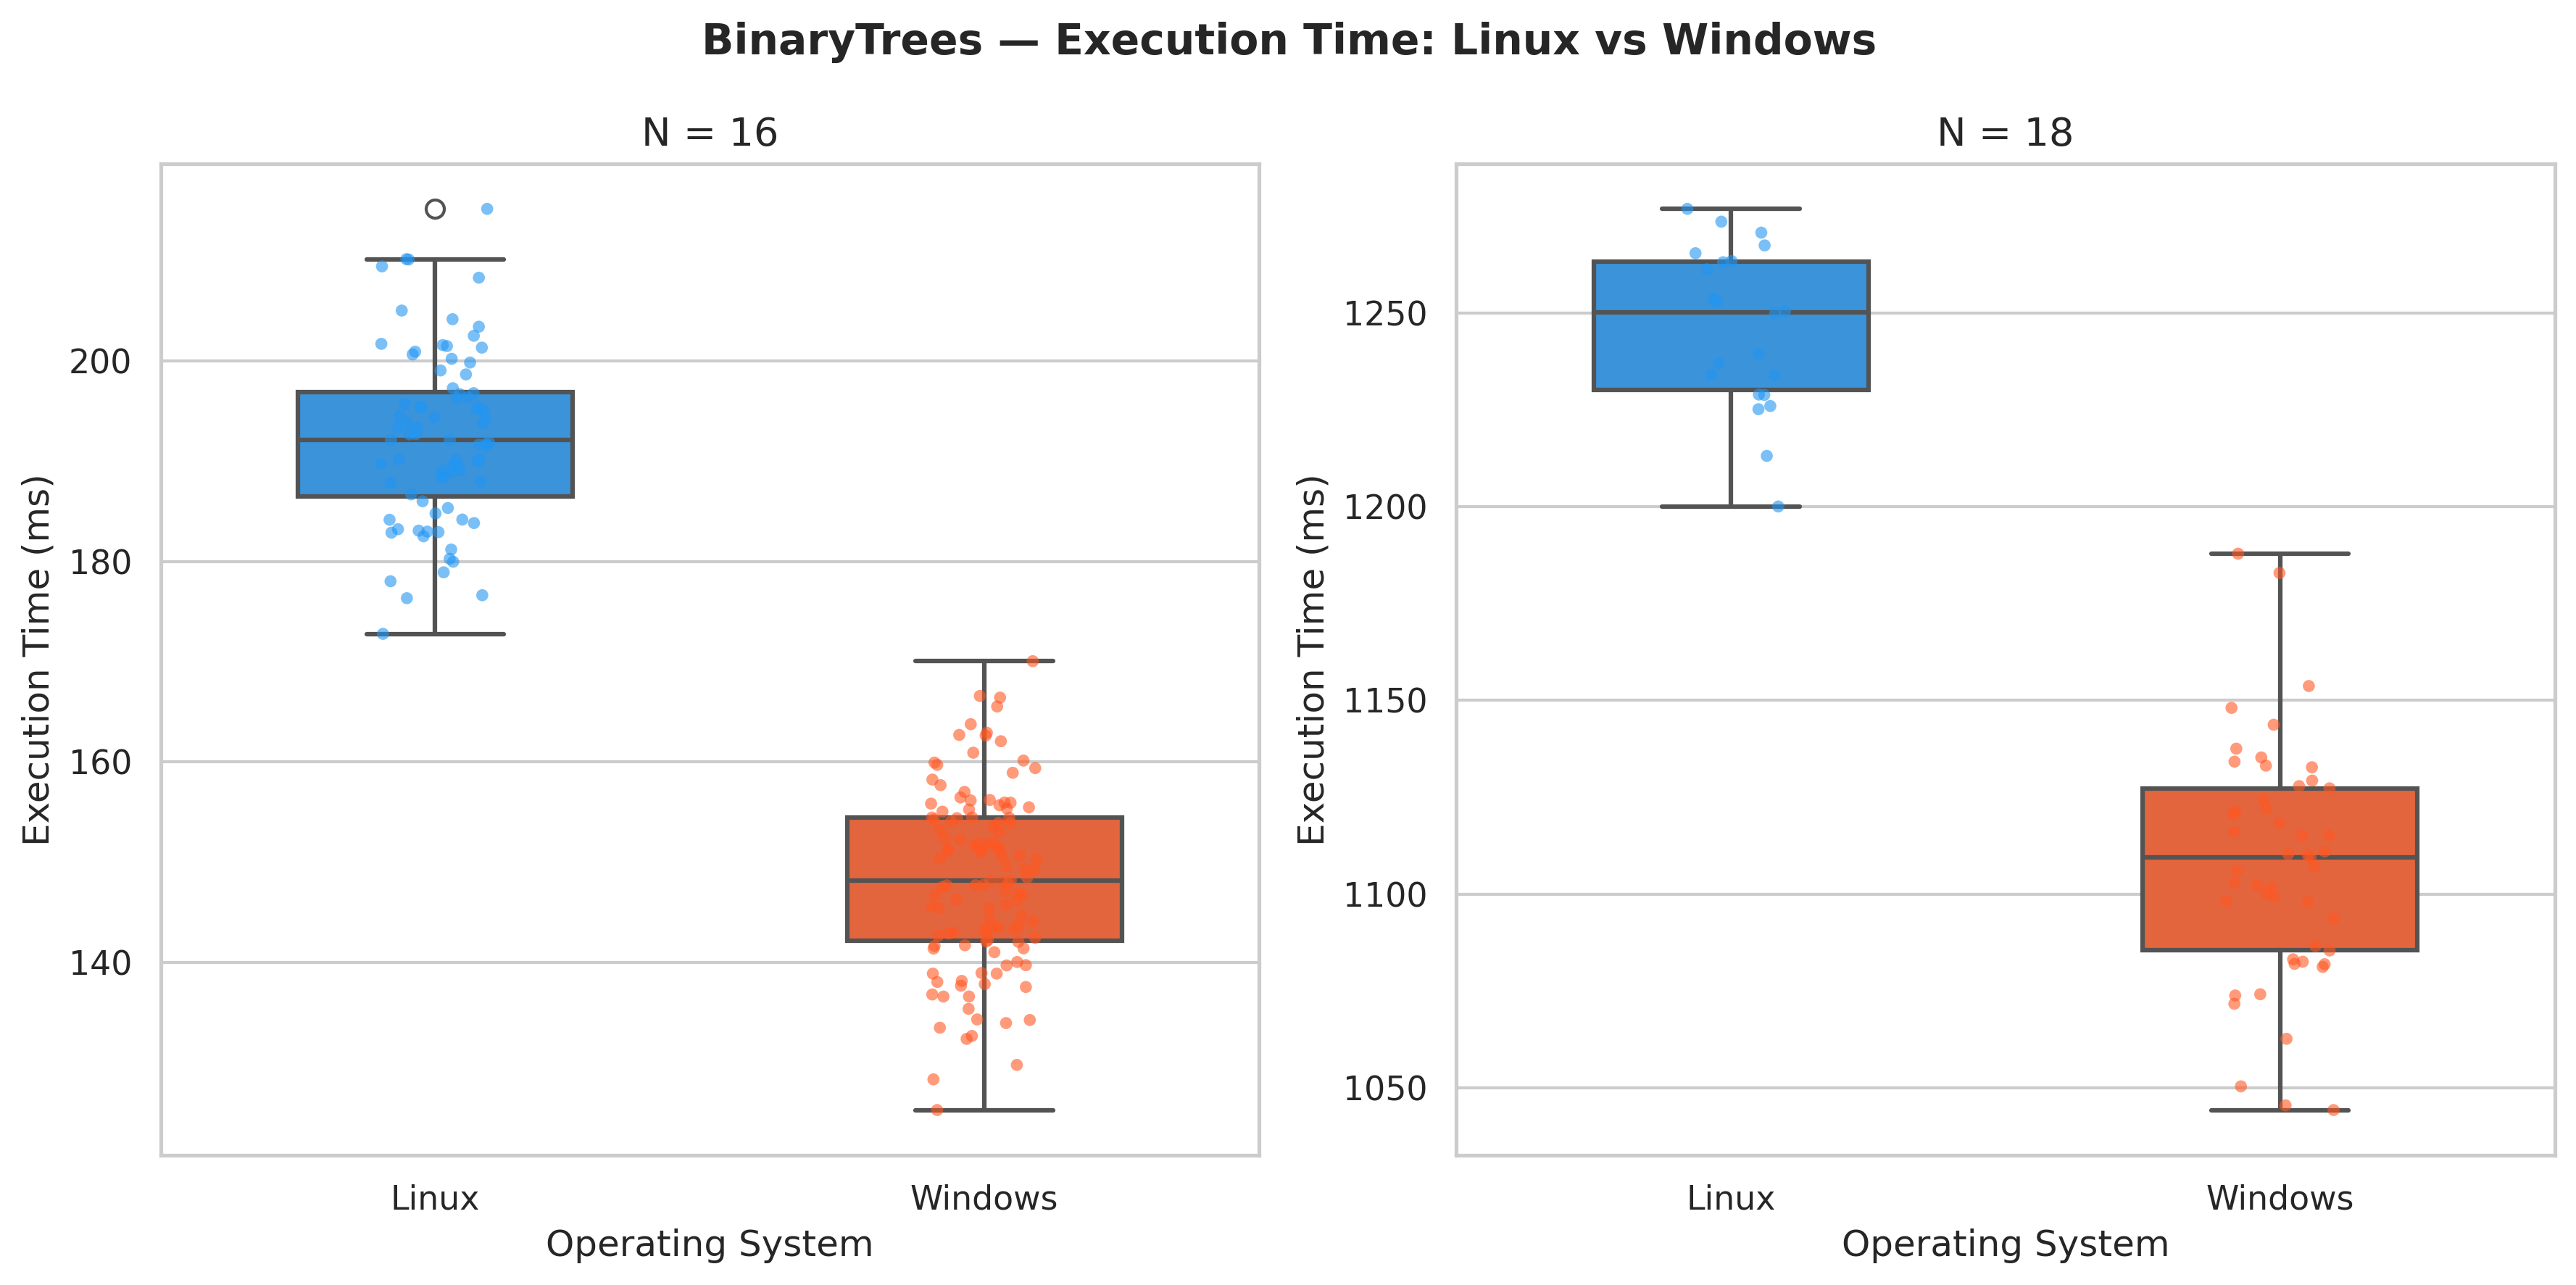
\includegraphics[width=\textwidth]{../analysis/figures/07_bt_boxplot_time.png}
  \caption{BinaryTrees: distribuição do tempo de execução para N=16 e N=18 em
    Linux e Windows.}
  \label{fig:bt_boxplot_time}
\end{figure}

A Figura~\ref{fig:bt_boxplot_energy} apresenta a distribuição do consumo
energético (domínio \textit{Package}) por SO e N.

\begin{figure}[H]
  \centering
  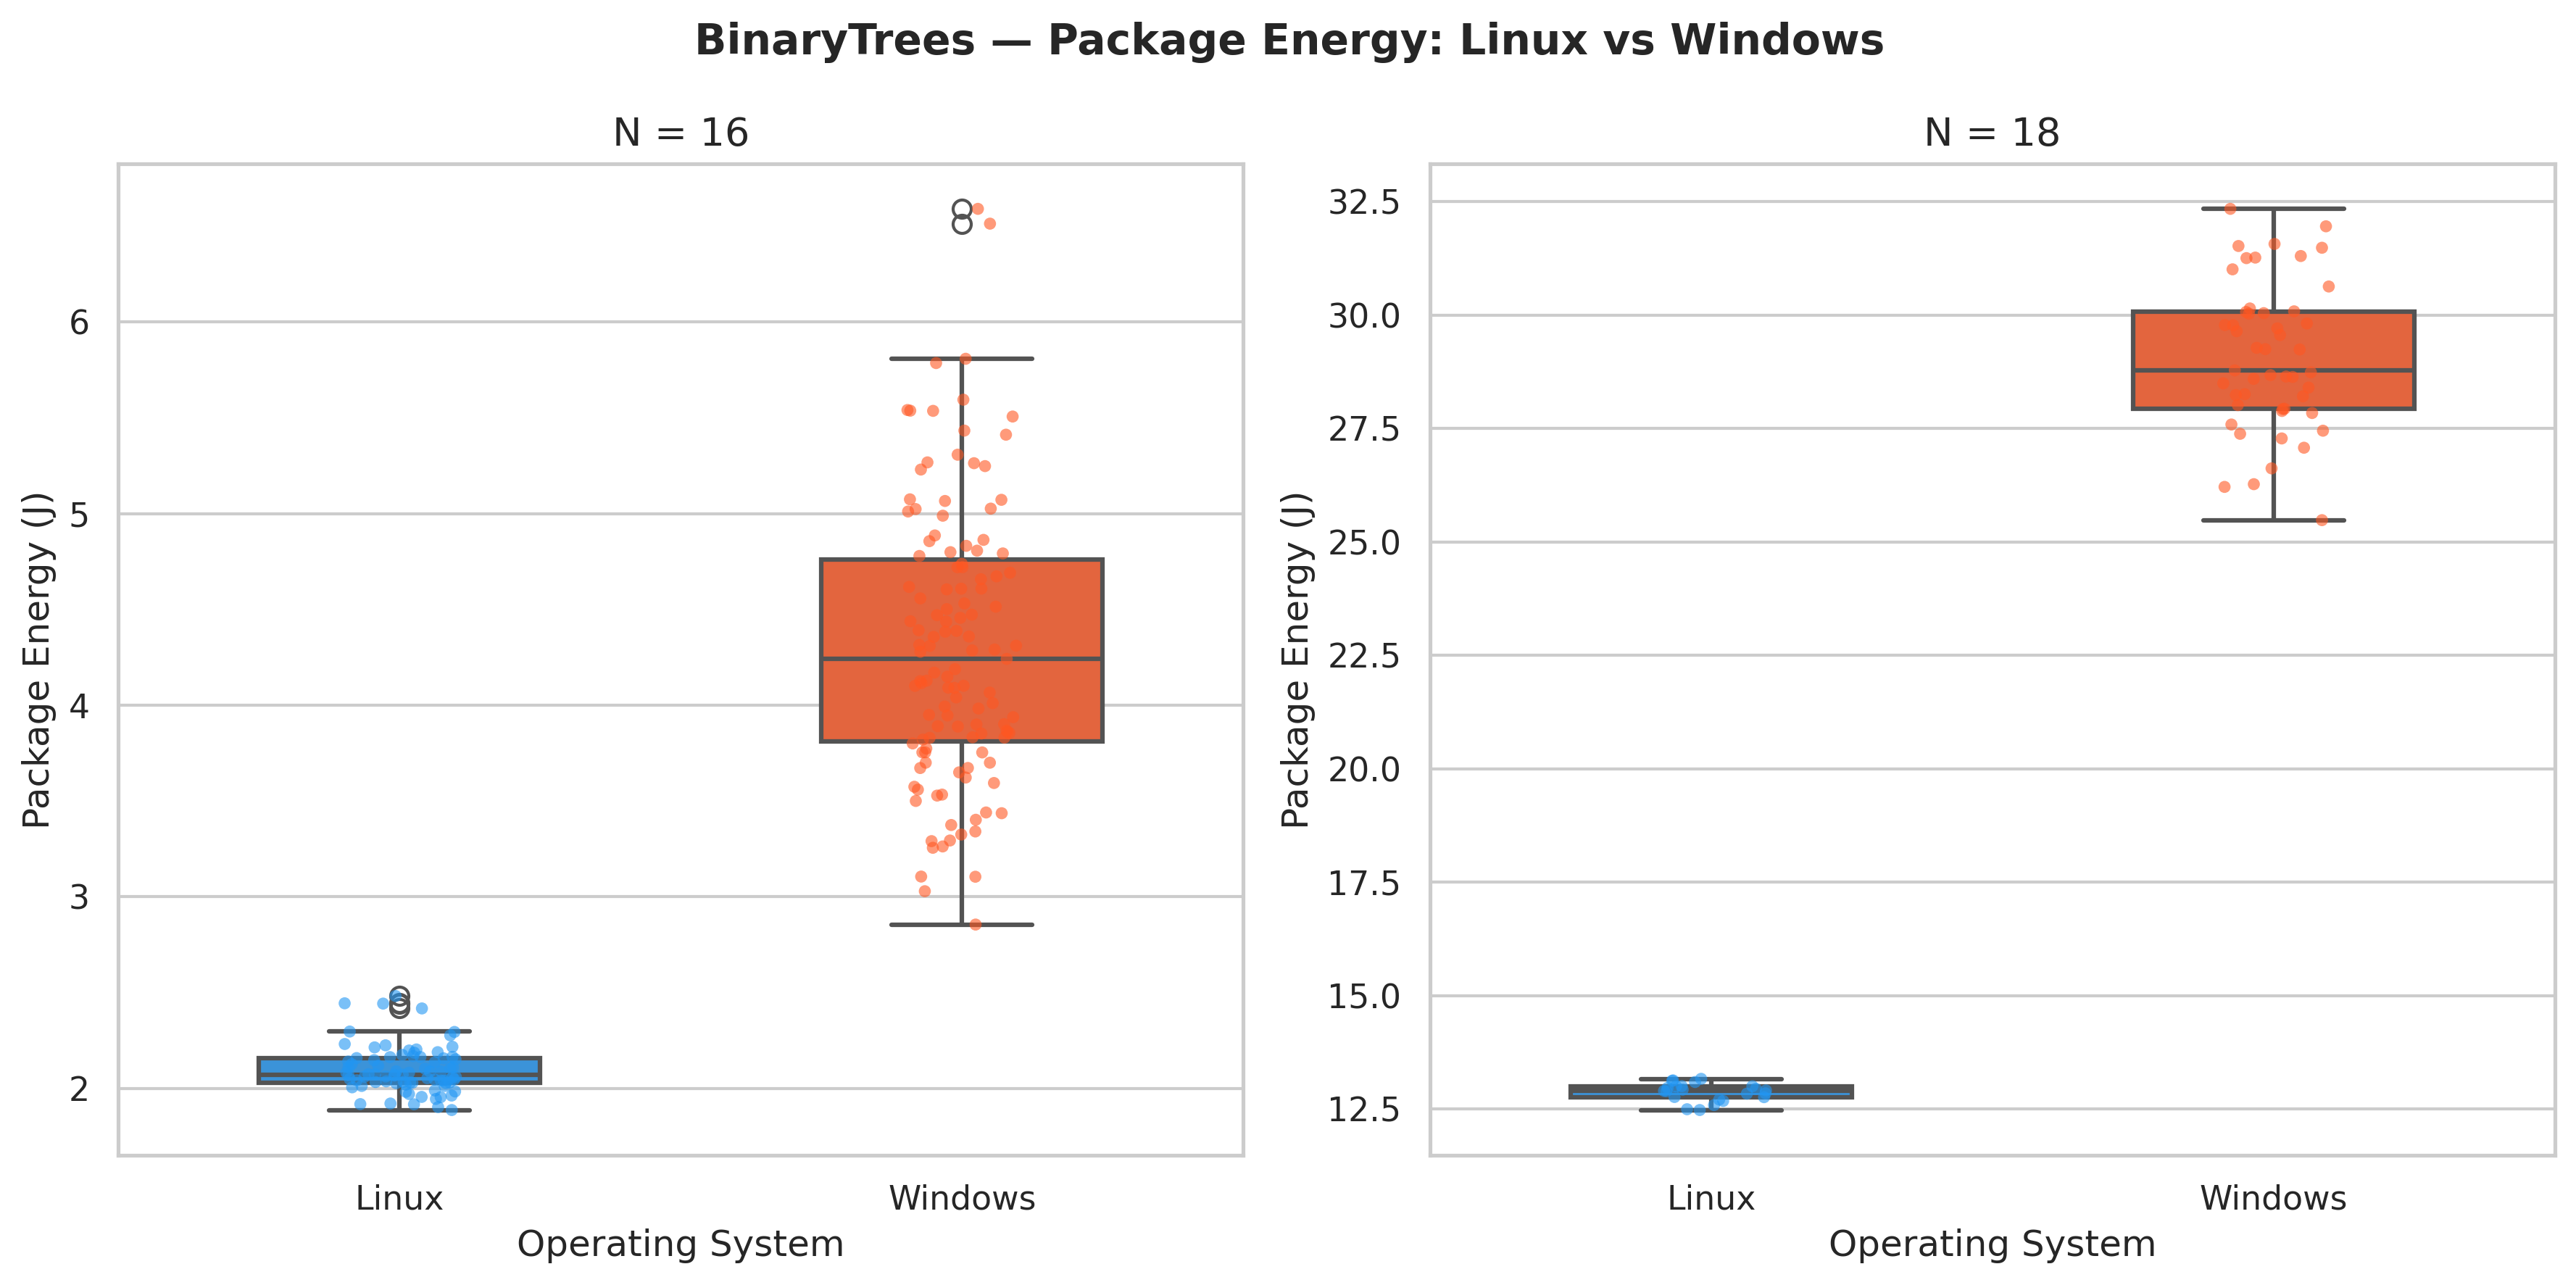
\includegraphics[width=\textwidth]{../analysis/figures/08_bt_boxplot_energy.png}
  \caption{BinaryTrees: distribuição do consumo energético (domínio
    \textit{Package}) para N=16 e N=18.}
  \label{fig:bt_boxplot_energy}
\end{figure}

\subsubsection{Comparação de Performance (Tempo)}

Para N=16, Windows executa em 148.3\,ms (IC 95\%: [146.7, 149.9]\,ms) vs.\
Linux 192.4\,ms (IC 95\%: [190.5, 194.3]\,ms).
\textbf{Windows é 22.8\% mais rápido} ($p < 0.001$).

Para N=18, Windows executa em 1107.8\,ms (IC 95\%: [1099.0, 1116.6]\,ms) vs.\
Linux 1246.1\,ms (IC 95\%: [1236.9, 1255.4]\,ms).
\textbf{Windows é 11.1\% mais rápido} ($p < 0.001$).

\subsubsection{Comparação de Consumo Energético}

Para N=16, Linux consome 2.097\,J (IC 95\%: [2.070, 2.123]\,J) vs.\ Windows
4.305\,J (IC 95\%: [4.176, 4.434]\,J).
\textbf{Linux consome 51.3\% menos energia} ($p < 0.001$).

Para N=18, Linux consome 12.878\,J (IC 95\%: [12.792, 12.965]\,J) vs.\ Windows
29.088\,J (IC 95\%: [28.624, 29.553]\,J).
\textbf{Linux consome 55.7\% menos energia} ($p < 0.001$).

\subsubsection{Significância Estatística}

A Tabela~\ref{tab:testes_bt} resume os testes de hipótese para BinaryTrees.
As diferenças no domínio \textit{Package} (tempo e energia) são todas
estatisticamente significativas com $p < 0.001$.
A diferença no domínio DRAM é significativa para N=18 mas não para N=16, o
que é consistente com o facto de a energia DRAM por iteração ser de apenas
0.21\,J em N=16 (próxima do limite de quantização do contador).

\begin{table}[H]
  \centering
  \caption{BinaryTrees: resultados dos testes de hipótese para tempo e
    energia.}
  \label{tab:testes_bt}
  \begin{tabular}{llllll}
    \toprule
    \textbf{N} & \textbf{Métrica} & \textbf{Teste} & \textbf{Estatística} &
    \textbf{p-value} & \textbf{Significativo} \\
    \midrule
    16 & Tempo        & Mann-Whitney U  & 9840.0     & $<$0.001 & Sim (***) \\
    16 & Energia Pkg  & Mann-Whitney U  & 0.0        & $<$0.001 & Sim (***) \\
    16 & Energia DRAM & Mann-Whitney U  & 4741.0     & 0.663    & Não       \\
    16 & Tempo        & Permutação A/B  & 44.1\,ms   & $<$0.001 & Sim (***) \\
    16 & Energia Pkg  & Permutação A/B  & $-$2.21\,J & $<$0.001 & Sim (***) \\
    18 & Tempo        & Mann-Whitney U  & 1078.0     & $<$0.001 & Sim (***) \\
    18 & Energia Pkg  & Mann-Whitney U  & 0.0        & $<$0.001 & Sim (***) \\
    18 & Energia DRAM & Mann-Whitney U  & 298.0      & 0.003    & Sim (**)  \\
    18 & Tempo        & Permutação A/B  & 138.4\,ms  & $<$0.001 & Sim (***) \\
    18 & Energia Pkg  & Permutação A/B  & $-$16.21\,J & $<$0.001 & Sim (***) \\
    \bottomrule
  \end{tabular}
\end{table}

\subsubsection{Correlação Tempo--Energia}

A correlação de Spearman entre tempo e energia em BinaryTrees é mais fraca no
\textit{dataset} combinado mas continua forte por SO, o que reflete o efeito do
GC sobre a relação tempo/energia:
\begin{itemize}
  \item Spearman $\rho$ (BinaryTrees completo) $= 0.318$, $p < 0.001$
  \item Spearman $\rho$ (Linux) $= 0.842$, $p < 0.001$
  \item Spearman $\rho$ (Windows) $= 0.721$, $p < 0.001$
\end{itemize}

\subsection{Análise do Domínio DRAM}
\label{sec:dram}

A Figura~\ref{fig:dram_comparison} compara o rácio
DRAM/\textit{Package} entre os dois \textit{benchmarks} e os dois SO.

\begin{figure}[H]
  \centering
  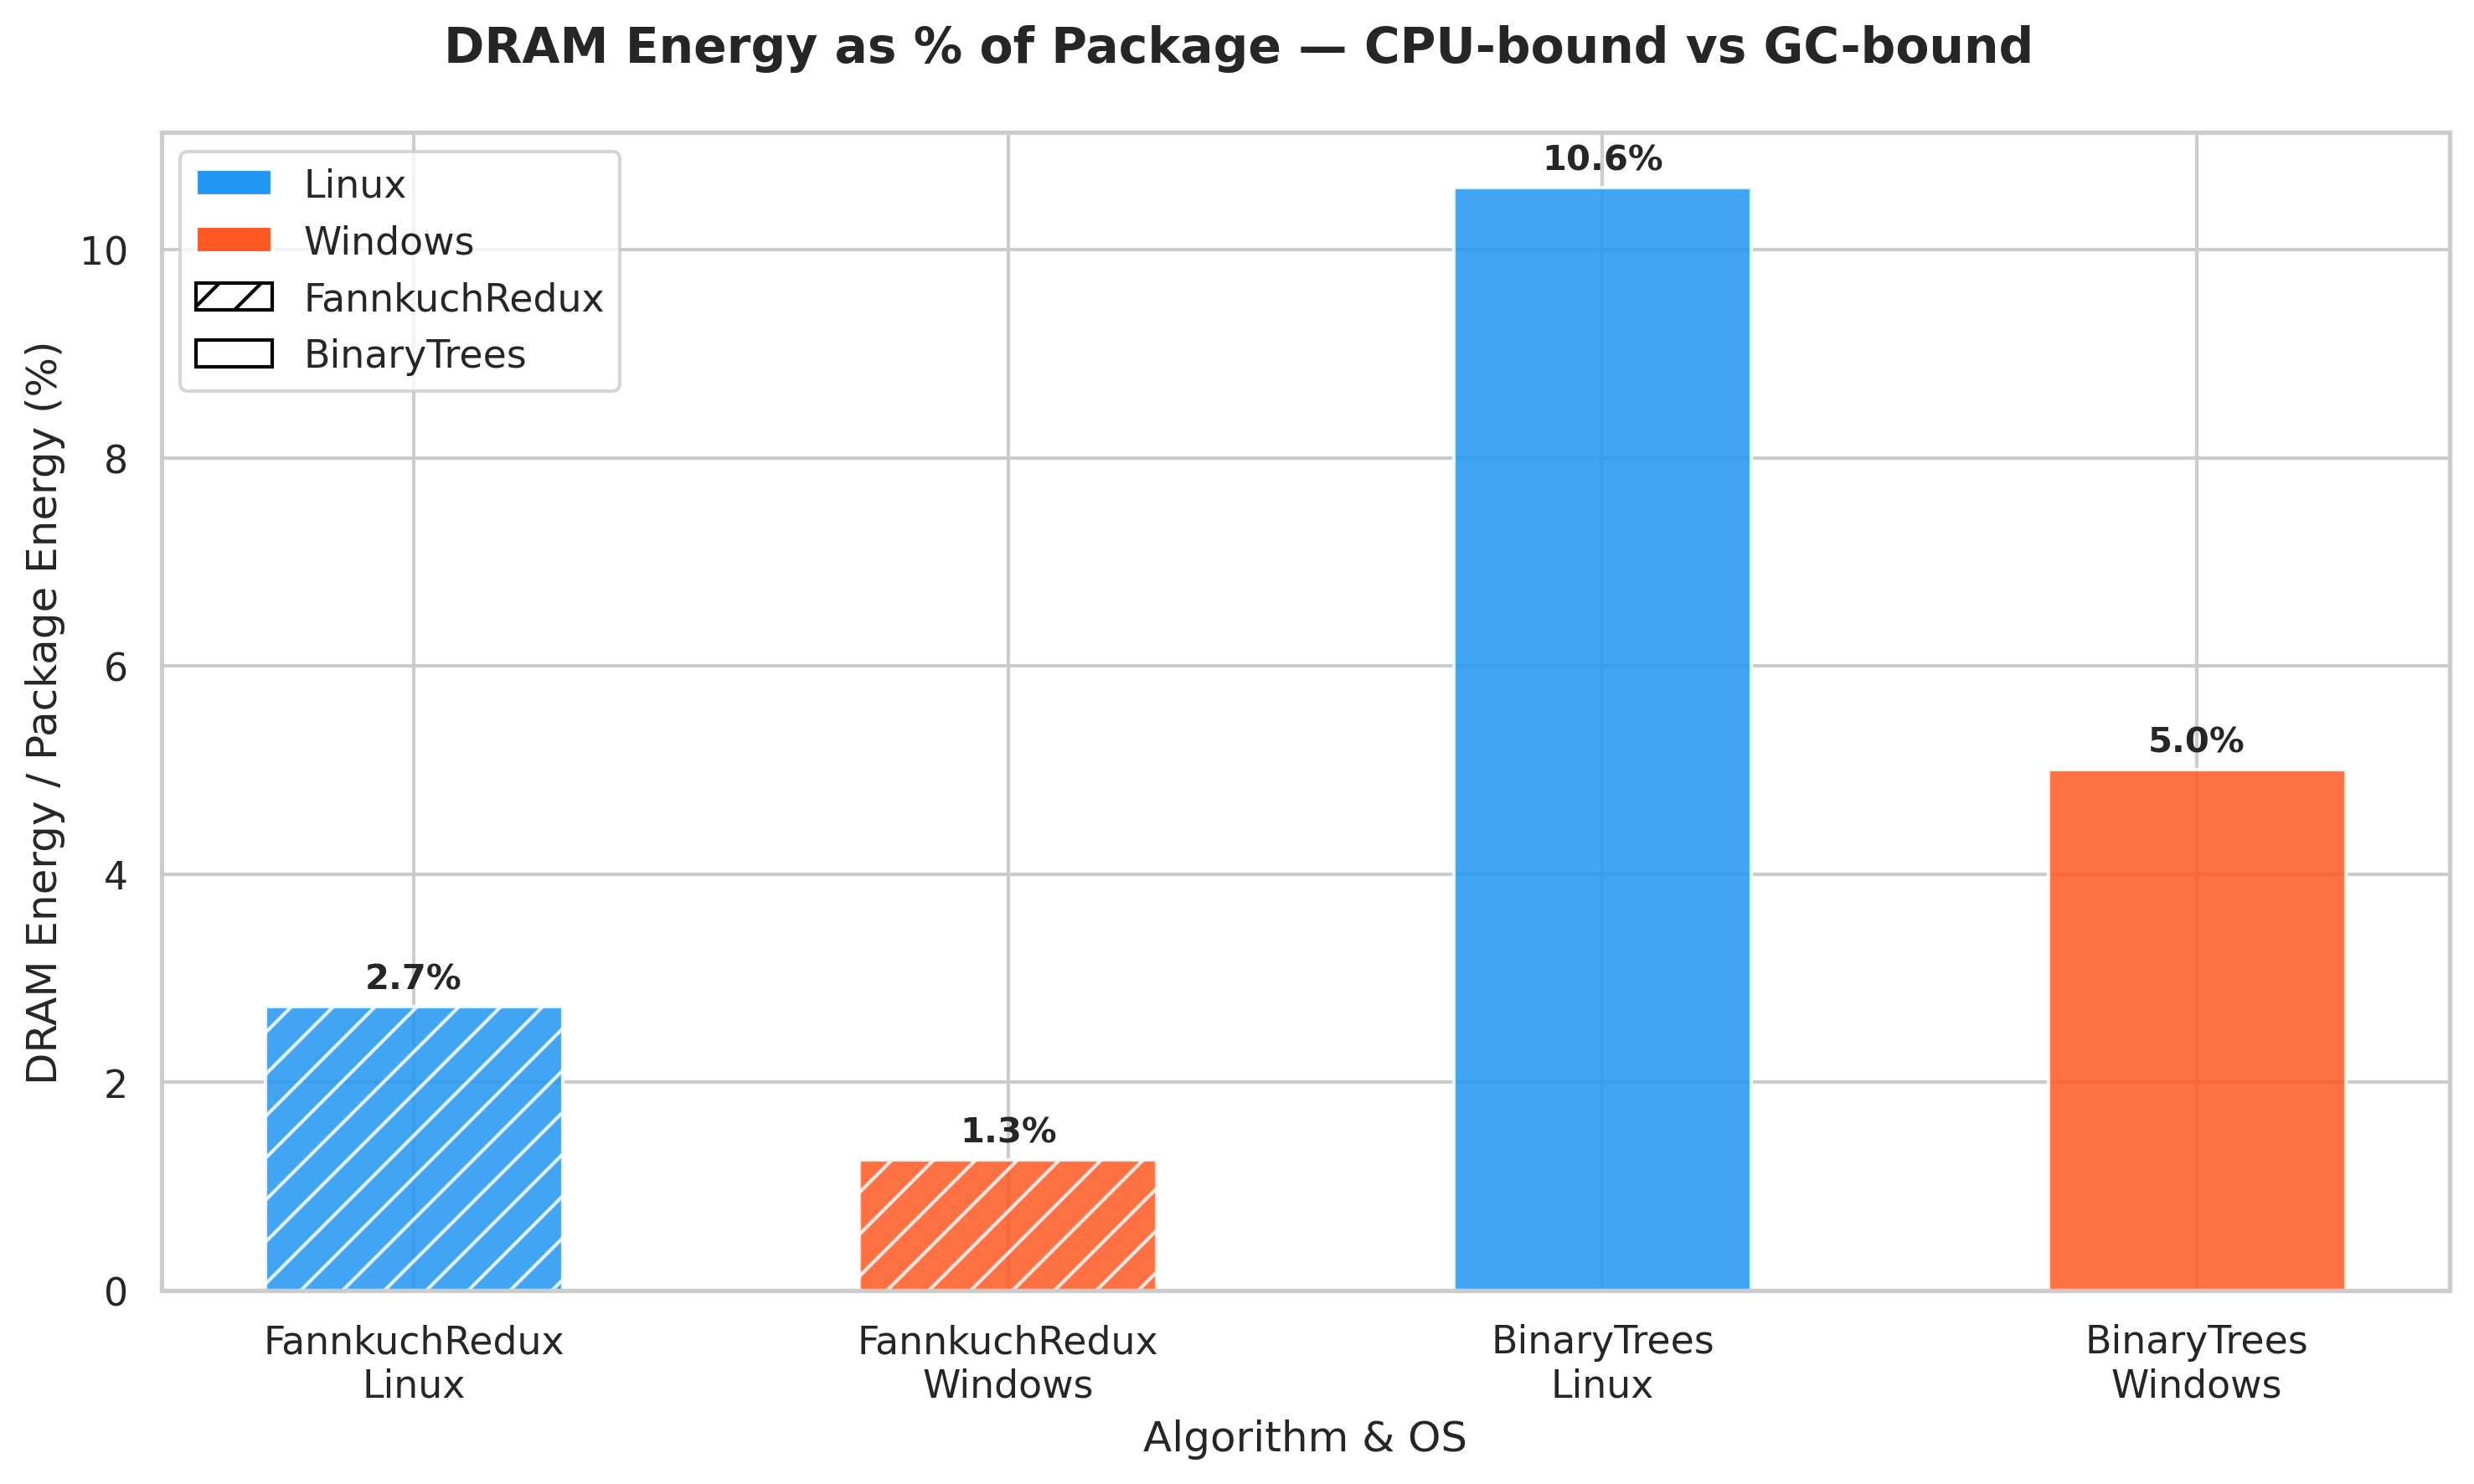
\includegraphics[width=\textwidth]{../analysis/figures/09_dram_comparison.png}
  \caption{Rácio DRAM/\textit{Package} (\%) por algoritmo e SO. BinaryTrees
    apresenta um rácio 4--8$\times$ superior ao FannkuchRedux, confirmando o
    seu perfil GC-bound / memory-bound.}
  \label{fig:dram_comparison}
\end{figure}

A medição independente do domínio DRAM produz uma assinatura clara para cada
\textit{workload}:
\begin{itemize}
  \item \textbf{FannkuchRedux:} DRAM representa 2.7\% da energia do
    \textit{Package} em Linux e 1.3\% em Windows.
  \item \textbf{BinaryTrees:} DRAM representa 10.6\% da energia do
    \textit{Package} em Linux e 5.0\% em Windows.
\end{itemize}

A diferença de 4--8$\times$ entre os dois algoritmos confirma
experimentalmente que BinaryTrees pressiona o subsistema de memória de forma
substancialmente superior, validando a sua classificação como
\textit{benchmark} GC-bound / memory-bound.
A diferença de rácio entre SO (Linux apresenta sempre rácio mais elevado) é
consistente em ambos os algoritmos e sugere que o domínio \textit{Package} no
Windows está a contabilizar consumo adicional fora do subsistema DRAM
(\textit{e.g.}, frequência/voltagem mais elevada nos núcleos), e não que a
DRAM consome menos em Windows --- de facto, em valores absolutos, a energia
DRAM é praticamente idêntica entre SO (\textit{e.g.}, 0.212\,J em Linux vs.\
0.214\,J em Windows para BinaryTrees N=16).

\subsection{Comparação Global entre Algoritmos}

A Figura~\ref{fig:algorithm_comparison} sintetiza, num único gráfico, a
comparação entre os dois algoritmos e os dois SO ao nível de tempo e energia
por iteração.

\begin{figure}[H]
  \centering
  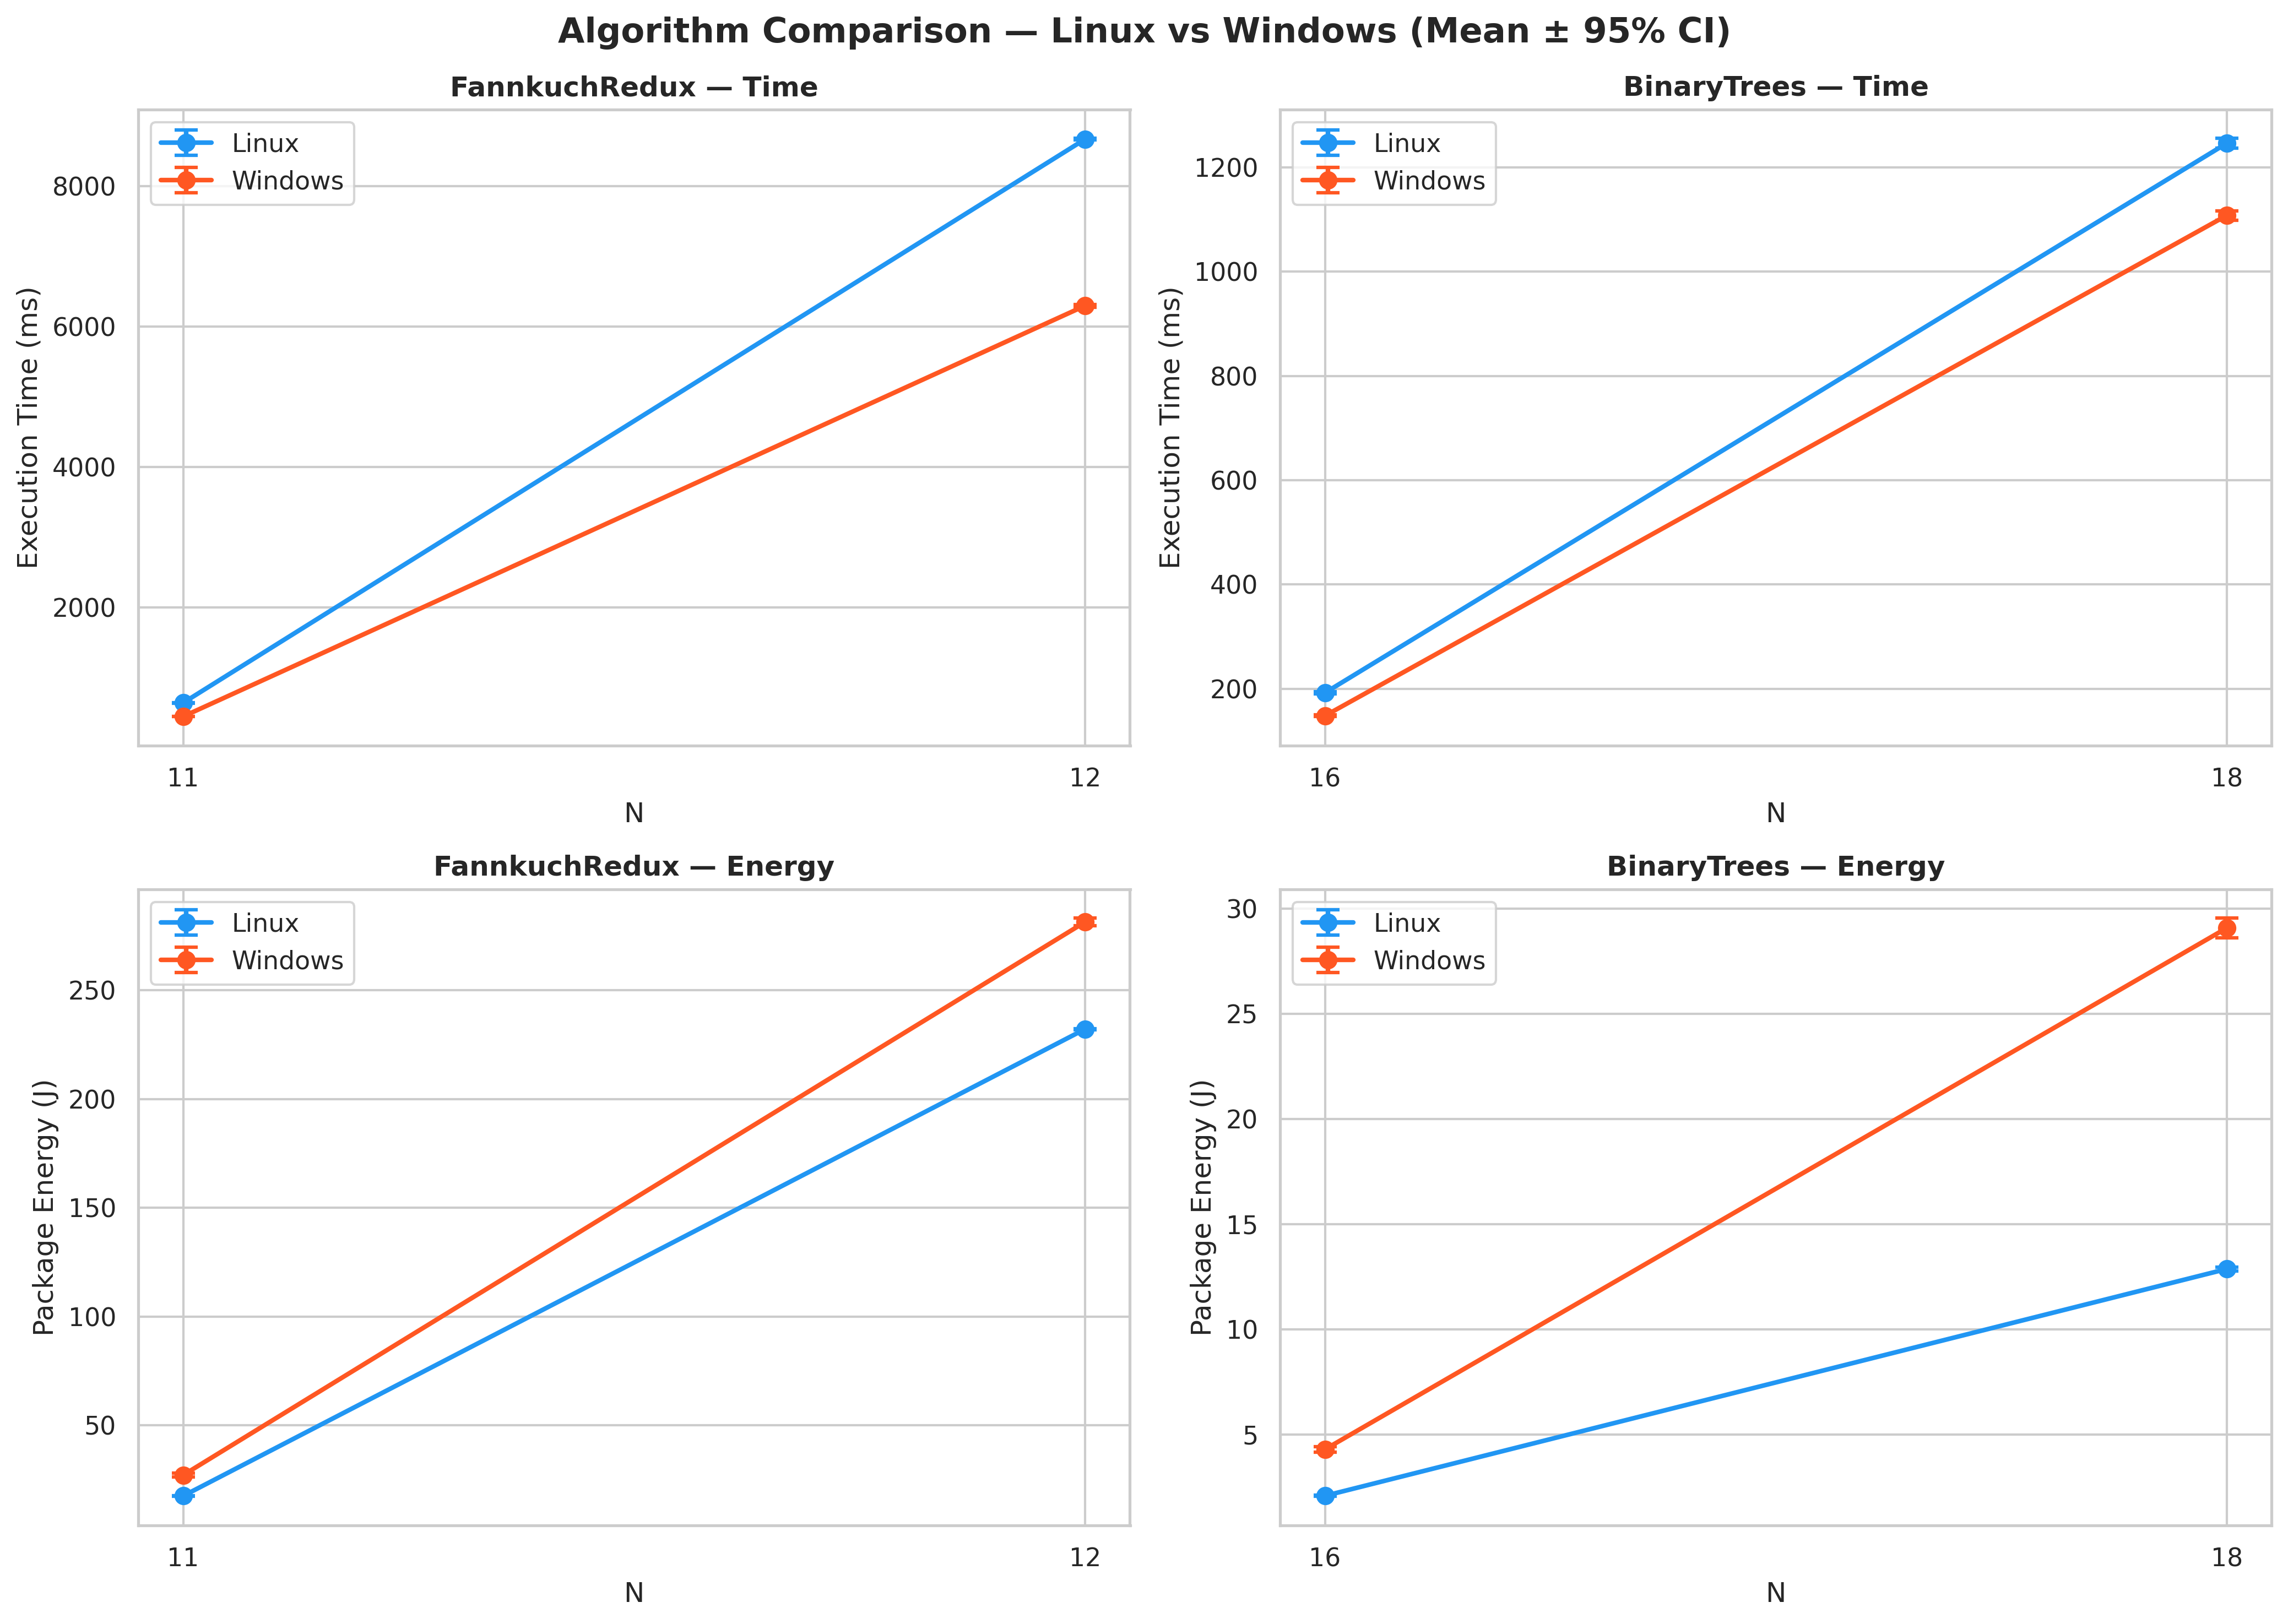
\includegraphics[width=\textwidth]{../analysis/figures/10_algorithm_comparison.png}
  \caption{Comparação global tempo vs.\ energia entre FannkuchRedux e
    BinaryTrees, por SO e N.}
  \label{fig:algorithm_comparison}
\end{figure}

%% ─────────────────────────────────────────────────────────────────────────────
\section{Discussão}
\label{sec:discussao}
%% ─────────────────────────────────────────────────────────────────────────────

\subsection{Windows é mais rápido --- porquê?}

Os algoritmos usam \texttt{Task.Run} com \textit{workers} dependentes do
número de núcleos.
O ThreadPool do Windows é historicamente mais agressivo a escalonar
\textit{threads} em múltiplos núcleos para \textit{workloads} curtas.
O .NET no Windows pode também beneficiar de otimizações específicas da
plataforma no JIT (RyuJIT x64).
Embora o turbo tenha sido desativado, diferenças residuais de frequência entre
os governadores de cada SO não podem ser completamente excluídas.
O \textit{scheduler} CFS do Linux (\textit{Completely Fair Scheduler}) prioriza
equidade sobre \textit{throughput} máximo, o que pode desfavorecer
\textit{workloads} multi-threaded intensivas.

\subsection{Linux consome menos energia --- porquê?}

Windows executa mais rápido, mas consome proporcionalmente mais energia em
ambos os \textit{benchmarks}.
Este resultado é contra-intuitivo se se assumir que ``mais rápido = menos
tempo a trabalhar = menos energia''.
A explicação mais provável é que Windows opera os núcleos a
voltagem/frequência mais elevada mesmo com turbo desativado (estados de
potência C0 mais agressivos, menor uso de C-states entre tarefas).
O governor \texttt{performance} do Linux mantém frequência base constante
($\approx$2.6\,GHz) com transições suaves de C-state.
O plano ``Desempenho Máximo'' do Windows pode operar em estados de potência
mais elevados de forma mais contínua.
Para \textit{workloads} onde o tempo de resposta não é crítico, Linux oferece
melhor eficiência energética.

\subsection{Trade-off velocidade vs.\ energia}

Existe um \textit{trade-off} claro: Windows oferece aproximadamente 11--43\%
mais velocidade em troca de 17--56\% mais consumo energético, dependendo do
algoritmo e de N.
A magnitude do efeito varia com a duração da \textit{run}: em FannkuchRedux,
para N=12 (\textit{workload} mais longa), a diferença de energia reduz-se em
relação a N=11 (17\% vs.\ 35\%), sugerindo que o efeito é mais pronunciado em
\textit{workloads} curtas onde os \textit{overheads} de \textit{scheduling}
dominam.
Para aplicações onde a eficiência energética é prioritária (\textit{e.g.},
servidores em \textit{data centers} com custo de energia elevado, dispositivos
embebidos), Linux apresenta vantagem clara.

\subsection{BinaryTrees vs.\ FannkuchRedux --- impacto do perfil de memória}
\label{sec:disc_perfil}

A comparação cruzada entre os dois \textit{benchmarks} revela um padrão
consistente:

\begin{itemize}
  \item \textbf{Vantagem de velocidade do Windows é menor em BinaryTrees}
    (11--23\%) do que em FannkuchRedux (38--43\%).
    A pressão de GC introduz pausas e custos de gestão de memória que parecem
    equalizar parcialmente a vantagem do \textit{scheduler} do Windows.
  \item \textbf{Vantagem de energia do Linux é maior em BinaryTrees}
    (51--56\%) do que em FannkuchRedux (17--35\%).
    Quando o subsistema de memória se torna dominante, a eficiência energética
    do Linux ganha ainda mais relevância.
  \item \textbf{O domínio DRAM confirma experimentalmente o perfil de memória
    distinto}: BinaryTrees apresenta um rácio DRAM/Package 4--8$\times$
    superior ao de FannkuchRedux (Secção~\ref{sec:dram}).
    Esta evidência por hardware (RAPL DRAM) é independente das estatísticas de
    \textit{heap} reportadas pelo \texttt{MemoryDiagnoser} e valida a
    classificação dos \textit{benchmarks}.
\end{itemize}

A leitura conjunta sugere que a pressão de GC \textit{atenua} as diferenças de
\textit{scheduler} entre SO mas \textit{amplifica} as diferenças de gestão de
energia: a vantagem de velocidade do Windows é menor (a CPU está parcialmente
à espera do GC e do subsistema de memória), mas o Windows continua a operar
em estados de potência mais elevados durante essas pausas, pelo que o consumo
energético cresce desproporcionalmente.

%% ─────────────────────────────────────────────────────────────────────────────
\section{Ameaças à Validade}
\label{sec:ameacas}
%% ─────────────────────────────────────────────────────────────────────────────

\subsection{Validade Interna}

\textbf{Sessões separadas:} as medições Linux e Windows foram realizadas em
momentos distintos.
Fatores como temperatura ambiente e estado do hardware podem introduzir
\textit{bias} sistemático.

\textbf{Temperatura Windows não disponível:} impossibilidade de correlacionar
temperatura com desempenho no Windows
(\texttt{cpu\_temp\_before}~$=$~\texttt{cpu\_temp\_after}~$=-1.0$).

\textbf{Filtro RAPL:} a Intel adicionou ruído aleatório às leituras RAPL
(IPU 2021.2) como mitigação de ataques \textit{side-channel}.
Afeta ambos os SO de forma equivalente; mitigado pelo número elevado de
iterações.

\subsection{Validade Externa}

\textbf{Hardware único:} os resultados foram obtidos num único \textit{laptop}
(HP EliteBook 1050 G1, i7-8850H) e podem não generalizar para outros
processadores (AMD, ARM) ou fatores de forma (desktop, servidor).

\textbf{Cobertura de algoritmos:} os \textit{benchmarks} cobrem dois perfis
distintos (CPU-bound e GC-bound), o que reforça as conclusões em relação à
versão anterior do estudo.
Resultados podem ainda diferir para \textit{workloads} com I/O intensivo ou
execução estritamente \textit{single-threaded}.

\textbf{Versão .NET:} testado com .NET 9.
Resultados podem variar com versões anteriores ou futuras.

\subsection{Validade de Construção}

\textbf{Dimensão da amostra:} as amostras válidas variam por grupo:
FannkuchRedux apresenta 19--25 amostras por grupo (limite mínimo do Teorema
do Limite Central, mas adequado para os testes não-paramétricos utilizados,
válidos para $n \geq 20$); BinaryTrees apresenta 22--123 amostras por grupo,
todas acima do limite recomendado.

\textbf{Oversampling de Windows N=16 em BinaryTrees:} o BenchmarkDotNet recolheu
123 amostras válidas para BinaryTrees N=16 em Windows (vs.\ 80 em Linux para
o mesmo grupo) por convergência mais lenta dos critérios de estabilidade
estatística da ferramenta.
Como as amostras são recolhidas de forma independente e os testes utilizados
(Mann-Whitney U, permutação) não exigem grupos equilibrados, o
\textit{oversampling} não afeta a validade das comparações --- aumenta apenas
a precisão da estimativa do grupo correspondente.

\textbf{Variância em BinaryTrees:} o CV de BinaryTrees (1.7\%--6.0\%) é
superior ao de FannkuchRedux ($<$2\%), reflexo do impacto não-determinístico
do GC e do subsistema de memória.
Os \textit{outliers} foram removidos pelo critério IQR antes dos testes.

%% ─────────────────────────────────────────────────────────────────────────────
\section{Conclusão}
\label{sec:conclusao}
%% ─────────────────────────────────────────────────────────────────────────────

Este trabalho comparou a performance e o consumo energético de C\# (.NET 9) em
Windows 11 e Ubuntu 24.04 usando dois \textit{benchmarks} complementares:
FannkuchRedux (CPU-bound) e BinaryTrees (GC-bound / memory-bound).
A energia foi medida por hardware via Intel RAPL nos domínios \textit{Package}
e DRAM, em ambos os SO, no mesmo computador (\textit{dual-boot}).

Os resultados mostram que Windows 11 é consistentemente mais rápido em ambos
os \textit{benchmarks} (38--43\% em FannkuchRedux, 11--23\% em BinaryTrees)
mas consome significativamente mais energia (17--35\% em FannkuchRedux,
51--56\% em BinaryTrees) que Ubuntu 24.04, nas mesmas condições de hardware.
A medição independente do domínio DRAM revela que BinaryTrees apresenta um
rácio DRAM/\textit{Package} 4--8$\times$ superior ao de FannkuchRedux,
confirmando experimentalmente o seu perfil GC-bound e validando a escolha do
par de \textit{benchmarks}.
Todas as diferenças relevantes são estatisticamente significativas
(Mann-Whitney U, $p < 0.001$) e confirmadas por testes de permutação
independentes.

Os resultados evidenciam um \textit{trade-off} claro entre velocidade e
eficiência energética dependente do SO, com magnitude que varia com o perfil
de memória do \textit{workload}: em \textit{workloads} GC-bound, a vantagem
de velocidade do Windows reduz-se mas a vantagem energética do Linux
amplifica-se.
Para aplicações onde o custo energético é prioritário --- como servidores em
larga escala ou sistemas embebidos --- Linux apresenta vantagem significativa.

Como trabalho futuro sugere-se:
(1) replicar o estudo noutros tipos de hardware (desktop, servidor, ARM);
(2) incluir \textit{workloads} \textit{single-threaded} e com I/O intensivo;
(3) comparar versões de .NET (8 vs.\ 9 vs.\ 10);
(4) avaliar o impacto do modo \texttt{GC Server} vs.\ \texttt{GC Workstation}
em \textit{workloads} GC-bound como BinaryTrees;
(5) investigar o impacto de diferentes configurações do \textit{scheduler}
Linux (CFS vs.\ EEVDF, \textit{tickless kernel}).

%% ─────────────────────────────────────────────────────────────────────────────
\bibliographystyle{plainnat}
\bibliography{relatorio}
%% ─────────────────────────────────────────────────────────────────────────────

\end{document}
